\chapter{Approximate Bayesian methods}\label{chap15}

\textit{Approximate Bayesian methods} are a family of techniques designed to handle situations where the likelihood function lacks an analytical expression, is highly complex, or the problem is high-dimensional, whether due to a large parameter space or a massive dataset \cite{martin2024approximating}. In the former case, traditional Markov Chain Monte Carlo (MCMC) and importance sampling algorithms fail to provide a solution. In the latter, these algorithms struggle to produce accurate estimates within a reasonable timeframe, unless users modify them (see Chapter~\ref{chap13}).

However, there is no free lunch, \textit{Approximate Bayesian methods} address these challenges at the cost of providing an approximation to the posterior distribution rather than the \textit{exact} posterior. Nonetheless, asymptotic results show that the approximation improves as the sample size increases.

In this chapter, I first present \textit{simulation-based approaches}, which are designed to address situations where the likelihood is highly complex and may lack an analytical solution. In the second part, I introduce \textit{optimization approaches}, which are intended to handle high-dimensional problems. Specifically, I discuss approximate Bayesian computation (ABC) and Bayesian synthetic likelihood (BSL), the two most common \textit{simulation-based approaches}. Then, I present integrated nested Laplace approximations (INLA) and \textit{variational Bayes} (VB), the two most common \textit{optimization approaches} for high-dimensional problems.

\section{Simulation-based approaches}\label{sec15_1}
Taking into account the fundamental equation for performing parameter inference in the Bayesian framework,  
\begin{align*}
	\pi(\boldsymbol{\theta} \mid \mathbf{y}) & \propto p(\mathbf{y} \mid \boldsymbol{\theta}) \times \pi(\boldsymbol{\theta}),
\end{align*}  
we see in Section \ref{sec51} that MCMC algorithms, such as the Gibbs sampler (Section \ref{sec511}) and Metropolis-Hastings (Section \ref{sec512}), require evaluation of the likelihood function \( p(\boldsymbol{y} \mid \boldsymbol{\theta}) \) in the posterior conditional distribution or the acceptance probability, respectively. This is also the case for importance sampling when calculating the importance weights (Section \ref{sec52}).  

Thus, what happens when the likelihood function does not have an analytical expression? This situation arises in many models involving unobserved heterogeneity (i.e., unobserved taste preferences), models defined by quantile functions (e.g., the g-and-k distribution), or dynamic equilibrium models (e.g., repeated game models).

\textit{Simulation-based algorithms} provide a Bayesian solution when we face this situation, namely, when the likelihood function lacks an analytical expression or is highly complex. The only requirement is that we must be able to simulate synthetic data from the model conditional on the parameters. Therefore, these algorithms obtain an approximation to the posterior draws by simulating from the prior distribution $\pi(\boldsymbol{\theta})$ and then using these draws to simulate from the likelihood $p(\mathbf{y} \mid \boldsymbol{\theta})$.

\subsection{Approximate Bayesian computation}\label{sec15_12}

\textit{Approximate Bayesian Computation} (ABC) is designed to handle inferential situations where the likelihood function \( p(\boldsymbol{y} \mid \boldsymbol{\theta}) \) is intractable or highly complex, $\boldsymbol{y}\in \mathbb{R}^N$. It was introduced in population genetics by \cite{tavare1997inferring, pritchard1999population} and later generalized by \cite{beaumont2002approximate}. The basic intuitive origin of ABC appears to have been introduced by \cite{rubin1984bayesianly}. A growing body of literature explores its applications in biology, cosmology, finance, economics, and other fields.

The requirement in ABC is the ability to simulate from the parametric model. The process begins by drawing samples from the prior distribution \( \pi({\boldsymbol{\theta}}) \) multiple times, $\boldsymbol{\theta}\in\mathbb{R}^K$, and then simulating data from the model given each \( {\boldsymbol{\theta}^{(s)}}, s=1,2,\dots,S \). The resulting synthetic data, \( \boldsymbol{z}^{(s)} \in \mathbb{R}^N \) is used to compute summary statistics \( \boldsymbol{\eta}(\boldsymbol{z}^{(s)}) \in \mathbb{R}^L, L\geq K \). These summary statistics are crucial for the performance of ABC and should be selected based on a thorough understanding of the model.  

Next, we compare the synthetic summary statistics with the observed summary statistics \( \boldsymbol{\eta}(\boldsymbol{y}) \) using a distance metric \( d\left\{ \boldsymbol\eta ({\boldsymbol y}),{\boldsymbol \eta }({\boldsymbol z}^{(s)})\right\} \), typically the Euclidean distance. We retain the prior draws that generate synthetic summary statistics closest to the observed ones, that is, \( d\left\{ \boldsymbol\eta ({\boldsymbol y}),{\boldsymbol \eta }({\boldsymbol z}^{(s)})\right\}\leq \epsilon \), forming an approximation of the posterior distribution \( \pi_{\epsilon}(\boldsymbol{\theta},\boldsymbol{z} \mid \boldsymbol{\eta}(\boldsymbol{y})) \).

The simplest algorithm is the accept/reject approximate Bayesian computation (ABC-AR) (see Algorithm \ref{ABC0}).

\begin{algorithm}
	\caption{Accept/reject ABC}\label{ABC0}
	\begin{algorithmic}[1]
		\For{\texttt{$s=1,\dots,S$}}
		\State Draw ${\boldsymbol {\theta} }^{s}$ from $\pi({ \boldsymbol{\theta} }),$
		\State Simulate ${\boldsymbol z}^{s}=(z_{1}^{s},z_{2}^{s},...,z_{n}^{s})^{\top}$ from the model, $p(\cdot|{\boldsymbol{\theta} }^{s})$
		\State Calculate
		$d_{(s)}=d\{{\boldsymbol\eta }({\boldsymbol y}),{\boldsymbol \eta }({\boldsymbol z}^{s})\}$
		\EndFor
		\State Order the distances $d_{(1)}\leq\cdots\leq d_{(S)}$
		\State Select all $\boldsymbol{\theta}^s$ such that $d_{(i)}\leq \epsilon$, where $\epsilon>0$ is the tolerance level. 
	\end{algorithmic}
\end{algorithm}

Note that the posterior distribution is conditional on the summary statistics \( \boldsymbol{\eta}(\boldsymbol{y}) \) and the tolerance parameter \( \epsilon \). This implies that we obtain an approximation to the target distribution \( \pi(\boldsymbol{\theta} \mid \boldsymbol{y}) \), that is \( \pi(\boldsymbol{\theta} \mid \boldsymbol{\eta}(\boldsymbol{y})) \), because \( \boldsymbol{\eta}(\boldsymbol{y}) \) is not a sufficient statistic in most cases, and \( \epsilon > 0 \), these conditions introduce bias \cite{blum2010approximate}. However, ABC performs well compared to full-likelihood approaches in low-dimensional parameter spaces \cite{beaumont2002approximate}.

Furthermore, \cite{frazier2018asymptotic} show in Theorems 1 and 2 that Bayesian consistency and asymptotic normality hold, provided that \( \epsilon \to 0 \) fast enough as \( N \to +\infty \). In particular, the requirement is that the proportion of accepted draws converges to 0 at a rate faster than \( N^{-K / 2} \). Additionally, Theorem 2 in \cite{frazier2018asymptotic} shows that \( 100(1 -\alpha)\% \) Bayesian credible regions using ABC have frequentist coverage of \( 100(1 -\alpha)\% \). 

We should note from these asymptotic results that ABC suffers from the \textit{curse of dimensionality}. Specifically, given a sample size of 1,000 and two parameters, the proportion of accepted draws should be 0.1\%, meaning we would require one million prior draws to obtain 1,000 posterior draws. On the other hand, if the number of parameters is three, we would require 31.62 million prior draws. This limitation of ABC has attracted attention; see Chapter 8 of \cite{sisson2018handbook} for some potential solutions.

It is a common practice in ABC to perform a regression adjustment after retaining the draws \cite{beaumont2002approximate, leuenberger2010bayesian, sisson2018handbook}. This adjustment reduces bias in posterior draws by performing a simple linear regression between the selected draws and the discrepancy between the observed and simulated summary statistics, \( {\theta}^{(s)}_k = \alpha_k + \left(\boldsymbol{\eta}(\boldsymbol{y}) - \boldsymbol{\eta}(\boldsymbol{z}^{(s)})\right)^{\top}\boldsymbol{\beta}_k + \mu^{(s)}_k, \ k=1,2,\dots,K \). Then, the posterior draws are adjusted using the slope estimate \( {\theta}^{\text{adj},(s)}_k = {\theta}^{(s)}_k - \left(\boldsymbol{\eta}(\boldsymbol{y}) - \boldsymbol{\eta}(\boldsymbol{z}^{(s)})\right)^{\top}\hat{\boldsymbol{\beta}}_k \). Other regression adjustment strategies are also used, such as local linear regression, ridge regression, and neural networks. See the \textit{abc} package in \textbf{R}.

The favorable asymptotic sampling properties of ABC rely on correct model specification. \cite{frazier2020model} demonstrate that when the assumed model is misspecified, the asymptotic behavior of ABC can deteriorate. In particular, the posterior shape becomes asymptotically non-Gaussian, and the behavior of the posterior mean remains generally unknown. Additionally, regression adjustment approaches can produce posteriors that differ significantly from their simpler accept/reject counterparts.

Given these concerns, testing model specification in ABC is essential. This can be done using simulated goodness-of-fit statistics \cite{bertorelle2010abc,lintusaari2017fundamentals}, predictive p-values \cite{bertorelle2010abc}, discrepancy diagnostics \cite{frazier2020model}, and asymptotic tests \cite{ramirez2024testing} to evaluate model adequacy.

The accept/reject ABC algorithm is inefficient, as all draws are independent; thus, there is no learning from previous draws. This intensifies the computational burden. Therefore, \cite{marjoram2003markov, wegmann2009efficient} introduced Markov Chain Monte Carlo ABC (ABC-MCMC) algorithms, and \cite{sisson2007sequential, drovandi2011estimation, del2012adaptive, lenormand2013adaptive} proposed sequential Monte Carlo approaches (ABC-SMC). However, results comparing ABC-MCMC and ABC-SMC with ABC-AR are controversial regarding computational efficiency \cite{bertorelle2010abc}. In addition, ABC-AR is very simple and easily allows parallel computing \cite{frazier2019approximate}. Nevertheless, ABC-SMC is now the recommended approach, as it does not require tuning the algorithm's tolerance \cite{martin2024approximating}, and there are open-source implementations that facilitate its use.

New developments in ABC have focused on using empirical measures calculated from the observed ($\hat{\mu}_n$) and synthetic ($\hat{\mu}_{\boldsymbol{\theta}}^{(s)}$) data to replace summary statistics. Thus, $d\left\{ \boldsymbol\eta ({\boldsymbol y}),{\boldsymbol \eta }({\boldsymbol z}^{(s)})\right\}$ is replaced by $\mathcal{D}\left\{ \hat{\mu}_n,\hat{\mu}_{\boldsymbol{\theta}}^{(s)}\right\}$, where the latter is a discrepancy measure, such as the Kullback-Leibler divergence \cite{jiang2018approximate}. However, \cite{drovandi2022comparison} found in their simulation exercises that the best-performing summary statistics approach performs at least as well as the best discrepancy-measure approaches. The key point is to select informative summary statistics.\\

\textbf{Example: g-and-k distribution for financial returns} 

The g-and-k distribution is a highly flexible distribution capable of capturing skewness and heavy tails through its parameters. This makes it particularly useful for modeling real-world data that deviate from normality, especially in fields like finance, where outliers are common. However, this distribution lacks a closed-form expression for its density function.

The g-and-k distribution is defined by its quantile function \cite{drovandi2011likelihood}. Specifically, it is specified through its inverse cumulative distribution function,

\[
Q(p\mid{\theta}) = F^{-1}(p\mid{\theta}),
\]

where \( F = P(U \leq u) \), and \( Q \) represents the \( p \)-quantile \cite{rayner2002numerical}. The quantile function of the g-and-k distribution is given by

\[
Q^{gk}\left\{z(p)\mid a, b, c, g, k\right\} = a + b\left[1 + c \frac{1 - \exp\left\{-gz(p)\right\}}{1 + \exp\left\{-gz(p)\right\}}\right] \left\{1 + z(p)^2\right\}^k z(p),
\]

where \( z(p) \) is the standard normal quantile function, and \( c = 0.8 \) is a commonly suggested value.

In the g-and-k distribution, \( a \) is the location parameter, and \( b \) is the scale parameter, controlling the dispersion. The parameters \( g \) and \( k \) determine the levels of skewness and kurtosis, respectively, while \( c \) modifies the impact of skewness, and is typically set to 0.8.

\cite{drovandi2011likelihood} propose a moving average of order one using a g-and-k distribution to model exchange rate log returns. In particular,  
\[
z_t = \epsilon_t + \theta_1\epsilon_{t-1}, \quad t=1,\dots,524,
\]  
where \(\epsilon_t \sim N(0,1)\).  

The values of \(z_t\) are then divided by \((1+\theta_1^2)^{1/2}\) to ensure that they marginally follow a standard normal distribution. Thus, simulating g-and-k data requires only substituting \(z_t\) into the quantile function.  

We model exchange rate log daily returns from USD/EUR one year before and after the WHO declared the COVID-19 pandemic on 11 March 2020. We use the dataset \textit{ExchangeRate.csv} from our GitHub repository. Our ABC implementation uses twelve summary statistics: the seven octiles, the interquartile range, robust measures of skewness and kurtosis, and the autocorrelations of order one and two (see \cite{drovandi2011likelihood} and code below). We adopt the prior distributions proposed by \cite{ramirez2024testing}, 
\begin{align*}
	\theta_1\sim U(-1,1), \ a\sim U(0,5) \ b\sim U(0,5)\\
	g\sim U(-5,5), \ k\sim U(-0.5, 5).
\end{align*}

We use the \textit{EasyABC} package in \textbf{R} to implement the ABC accept/reject (ABC-AR) algorithm using 150,000 prior draws with an acceptance rate of 0.67\%. We also apply the ABC Markov chain Monte Carlo (ABC-MCMC) method \cite{marjoram2003markov} and the sequential Monte Carlo ABC (ABC-SMC) method \cite{lenormand2013adaptive} to compare the results across different ABC algorithms.\footnote{Note that this setting does not satisfy the asymptotic requirements for Bayesian consistency. However, it serves as a pedagogical exercise.} We generate 100,000 samples and retain 1\% in ABC-MCMC, and 30,000 samples, keeping 3.4\%, with a stopping criterion of 5\% in ABC-SMC. These settings imply that the three algorithms require approximately the same computational time. As ABC is a simulation-based method, the computational burden is mostly driven by the speed of simulating the process; thus, the \textit{EasyABC} package has parallel computing algorithms to speed up the processes. Users can refer to the cited references for algorithmic details, and the \textit{EasyABC} package for parallel computing implementation. 

In Exercise 1, we ask to program the ABC accept/reject algorithm (Algorithm \ref{ABC0}) from scratch and compare the results with those obtained using the ABC-AR implementation in the \textit{EasyABC} package.

The following code presents the results, and Figure \ref{figABCexc} compares the posterior distributions of $\theta_1$, $g$, and $k$ using the three methods. In this figure, we observe that ABC-MCMC (red) and ABC-SMC (green) exhibit similar performance, and both approaches provide more information than ABC-AR (blue). There is marginal positive evidence that the moving average coefficient is positive, and the three algorithms yield similar means, although ABC-AR exhibits lower precision. Since the posterior distribution of $g$ is centered around zero, the distribution appears to be symmetric around its median. Meanwhile, a positive $k$ indicates that the distribution has heavier tails than a normal distribution, implying a higher likelihood of extreme values (outliers) in the exchange rate USD/EURO.

\begin{tcolorbox}[enhanced,width=4.67in,center upper,
	fontupper=\large\bfseries,drop shadow southwest,sharp corners]
	\textit{R code. Exchange rate log returns: Approximate Bayesian computation}
	\begin{VF}
		\begin{lstlisting}[language=R]
######### ABC Exchange rate og returns: USD/EURO
rm(list = ls()); set.seed(010101)
library(EasyABC)
dfExcRate <- read.csv(file = "https://raw.githubusercontent.com/BEsmarter-consultancy/BSTApp/refs/heads/master/DataApp/ExchangeRate.csv", sep = ",", header = T)
attach(dfExcRate); n <- length(USDEUR)
# Summary statistics
SumSt <- function(y) {
	Oct <- quantile(y, c(0.125, 0.25, 0.375, 0.5, 0.625, 0.75, 0.875))
	eta1 <- Oct[6] - Oct[2]
	eta2 <- (Oct[6] + Oct[2] - 2 * Oct[4]) / eta1
	eta3 <- (Oct[7] - Oct[5] + Oct[3] - Oct[1]) / eta1
	autocor <- acf(y, lag = 2, plot = FALSE)
	autocor[["acf"]][2:3]
	Etay <- c(Oct, eta1, eta2, eta3, autocor[["acf"]][2:3])
	return(Etay)
}
# g-and-k distribution
RGKnewSum <- function(par) {
	z <- NULL
	theta <- par[1]; a <- par[2]; b <- par[3]; g <- par[4]; k <- par[5]
	e <- rnorm(n + 1)
	for(t in 2:(n + 1)){
		zt <- e[t] + theta * e[t-1]
		z <- c(z, zt)
	}
	zs <- z / (1 + theta^2)^0.5
	x <- a + b * (1 + 0.8 * (1 - exp(-g * zs)) / (1 + exp(-g * zs))) * (1 + zs^2)^k * zs
	Etaz <- SumSt(x)
	return(Etaz)
}
toy_prior <- list(c("unif",-1,1), c("unif",0,5), c("unif", 0,5), c("unif", -5,5), c("unif", -0.5,5))
sum_stat_obs <- SumSt(USDEUR)
tick <- Sys.time()
ABC_AR <- ABC_rejection(model=RGKnewSum, prior=toy_prior, summary_stat_target = sum_stat_obs, nb_simul=150000, tol = 0.0067,
progress_bar = TRUE)
tock <- Sys.time()
tock - tick
PostABCAR <- coda::mcmc(ABC_AR$param)
summary(PostABCAR)
tick <- Sys.time()
ABC_MCMC <- ABC_mcmc(method="Marjoram", model=RGKnewSum, prior=toy_prior, summary_stat_target=sum_stat_obs, n_rec = 100000, progress_bar = TRUE)
tock <- Sys.time()
tock - tick
PostABCMCMC <- coda::mcmc(ABC_MCMC[["param"]][order(ABC_MCMC[["dist"]])[1:1000],])
summary(PostABCMCMC)
tick <- Sys.time()
\end{lstlisting}
	\end{VF}
\end{tcolorbox}

\begin{tcolorbox}[enhanced,width=4.67in,center upper,
	fontupper=\large\bfseries,drop shadow southwest,sharp corners]
	\textit{R code. Exchange rate log returns: Approximate Bayesian computation}
	\begin{VF}
		\begin{lstlisting}[language=R]
ABC_SMC<-ABC_sequential(method="Lenormand", model=RGKnewSum, prior=toy_prior, summary_stat_target=sum_stat_obs, nb_simul = 30000, alpha = 0.034, p_acc_min = 0.05,
progress_bar = TRUE)
summary(PostABCSMC)
tock <- Sys.time()
tock - tick
PostABCSMC <- coda::mcmc(ABC_SMC[["param"]])
# Figures 
library(ggplot2); library(latex2exp)
Sp <- 1000

df1 <- data.frame(Value = c(PostABCAR[1:Sp,1], PostABCMCMC[1:Sp,1], PostABCSMC[1:Sp,1]),
Distribution = factor(c(rep("AR", Sp), rep("MCMC", Sp), rep("SMC", Sp))))
dentheta <- ggplot(df1, aes(x = Value, color = Distribution)) +   geom_density(linewidth = 1) + labs(title = TeX("Posterior density plot: $theta$"), x = TeX("$theta$"), y = "Posterior density") + scale_color_manual(values = c("blue", "red", "green")) +  theme_minimal() + theme(legend.title = element_blank())

df2 <- data.frame(Value = c(PostABCAR[1:Sp,4], PostABCMCMC[1:Sp,4], PostABCSMC[1:Sp,4]),
Distribution = factor(c(rep("AR", Sp), rep("MCMC", Sp), rep("SMC", Sp))))
deng <- ggplot(df2, aes(x = Value, color = Distribution)) +   geom_density(linewidth = 1) + labs(title = "Posterior density plot: g", x = "g", y = "Posterior density") +
scale_color_manual(values = c("blue", "red", "green")) +  theme_minimal() + theme(legend.title = element_blank())

df3 <- data.frame(Value = c(PostABCAR[1:Sp,5], PostABCMCMC[1:Sp,5], PostABCSMC[1:Sp,5]),
Distribution = factor(c(rep("AR", Sp), rep("MCMC", Sp), rep("SMC", Sp))))
denk <- ggplot(df3, aes(x = Value, color = Distribution)) +   geom_density(linewidth = 1) + labs(title = "Posterior density plot: k", x = "k", y = "Posterior density") +
scale_color_manual(values = c("blue", "red", "green")) +  theme_minimal() + theme(legend.title = element_blank())

library(ggpubr)
ggarrange(dentheta, deng, denk, labels = c("A", "B", "C"), ncol = 3, nrow = 1,
legend = "bottom", common.legend = TRUE)
\end{lstlisting}
	\end{VF}
\end{tcolorbox}

\begin{figure}[!h]
	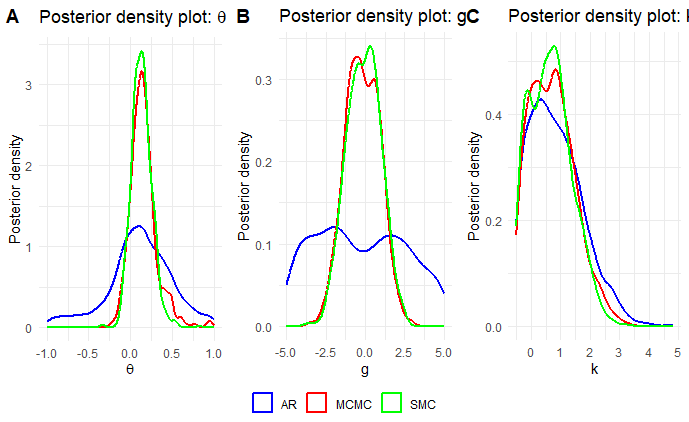
\includegraphics[width=340pt, height=200pt]{Chapters/chapter15/figures/ABCexcrate.png}
	\caption[List of figure caption goes here]{Posterior distributions using approximate Bayesian computation: Exchange rate log returns USD/EURO.}\label{figABCexc}
\end{figure}

\subsection{Bayesian synthetic likelihood}\label{sec15_13}

Note that in ABC, in most cases, we target the posterior distribution $\pi(\boldsymbol{\theta} \mid \boldsymbol{\eta}(\boldsymbol{y}))$ rather than $\pi(\boldsymbol{\theta} \mid \boldsymbol{y})$, as $\boldsymbol{\eta}(\boldsymbol{y})$ is not a sufficient statistic, $\boldsymbol{y}\in \mathbb{R}^N$, $\boldsymbol{\theta}\in \mathbb{R}^K, \ \boldsymbol{\eta}(\boldsymbol{y})\in \mathbb{R}^L, \ L\geq K$. This can be beneficial since discarding information may improve the behavior of the likelihood or make the inference more robust to model misspecification \cite{price2018bayesian}. Given the intractability of $p(\boldsymbol{y} \mid \boldsymbol{\theta})$, it is highly likely that $p(\boldsymbol{\eta}(\boldsymbol{y}) \mid \boldsymbol{\theta})$ is also intractable. \cite{wood2010statistical} addressed this issue by introducing an auxiliary model for the summary statistics, assuming $p_a(\boldsymbol{\eta}(\boldsymbol{y})\mid \boldsymbol{\theta}) = N(\boldsymbol{\mu}_{\boldsymbol{\theta}}, \boldsymbol{\Sigma}_{\boldsymbol{\theta}})$.

Bayesian synthetic likelihood (BSL) arises when this auxiliary likelihood is combined with a prior distribution on the parameter \cite{drovandi2015bayesian,price2018bayesian},
\begin{align*} 
	\pi_{a}(\boldsymbol{\theta} \mid \boldsymbol{\eta}(\boldsymbol{y})) &\propto p_{a}(\boldsymbol{\eta}(\boldsymbol{y})\mid \boldsymbol{\theta}) \pi(\boldsymbol{\theta}), 
\end{align*}

where the subscript \( a \) indicates that this is an approximation due to the Gaussian assumption. This is referred to as the idealized BSL posterior. However, note that \( p_a(\boldsymbol{\eta}(\boldsymbol{y})\mid \boldsymbol{\theta}) \) is rarely available, as \( \boldsymbol{\mu}_{\boldsymbol{\theta}} \) and \( \boldsymbol{\Sigma}_{\boldsymbol{\theta}} \) are generally unknown. Therefore, we estimate these quantities using simulations from the model given a realization of $\boldsymbol{\theta}$:\footnote{There are better ways to calculate the covariance matrix, see \cite{nott2023bayesian}.}
\begin{align*} 
	\widehat{\boldsymbol{\mu}}_{\boldsymbol{\theta}} &= \frac{1}{M} \sum_{m=1}^{M} \boldsymbol{\eta}(\boldsymbol{z}^{(m)}),\\
	\widehat{\boldsymbol{\Sigma}}_{\boldsymbol{\theta}} &= \frac{1}{M-1} \sum_{m=1}^{M} (\boldsymbol{\eta}(\boldsymbol{z}^{(m)}) - \widehat{\boldsymbol{\mu}}_{\boldsymbol{\theta}})(\boldsymbol{\eta}(\boldsymbol{z}^{(m)}) - \widehat{\boldsymbol{\mu}}_{\boldsymbol{\theta}})^{\top}. 
\end{align*}

Then, we have 
\begin{align*} 
	\pi_{a,M}(\boldsymbol{\theta} \mid \boldsymbol{\eta}(\boldsymbol{y})) &\propto p_{a,M}(\boldsymbol{\eta}(\boldsymbol{y})\mid \boldsymbol{\theta}) \pi(\boldsymbol{\theta}), 
\end{align*}
where $p_{a,M}(\boldsymbol{\eta}(\boldsymbol{y}))$ uses the estimates, which in turn depends on the number of draws $M$ to calculate $\widehat{\boldsymbol{\mu}}_{\boldsymbol{\theta}}$ and $\widehat{\boldsymbol{\Sigma}}_{\boldsymbol{\theta}}$. Note that although we can have unbiased estimators of these object, in general, $N(\boldsymbol{\eta}(\boldsymbol{y})\mid \widehat{\boldsymbol{\mu}}_{\boldsymbol{\theta}},\widehat{\boldsymbol{\Sigma}}_{\boldsymbol{\theta}})$ is not an unbiased estimator of $N(\boldsymbol{\eta}(\boldsymbol{y})\mid {\boldsymbol{\mu}}_{\boldsymbol{\theta}},{\boldsymbol{\Sigma}}_{\boldsymbol{\theta}})$. \cite{an2022bsl} show an unbiased estimator for BSL. 

\cite{nott2023bayesian} show that \( \pi_{a,M}(\boldsymbol{\theta}) \) converges asymptotically to a Gaussian distribution and that the \( 100(1-\alpha)\% \) Bayesian credible regions using BSL have frequentist coverage of \( 100(1-\alpha)\% \). In addition, the posterior mean from BSL is also asymptotically Gaussian. These results require convenient estimation of the covariance matrix and that \( M \to \infty \) as \( N \to \infty \), $M=C\lfloor N^{\gamma} \rfloor, \ C>0, \ \gamma > 0$ and $\lfloor x \rfloor$ denoting the integer floor of $x$. Thus, the choice of \( M \) does not drastically affect the desirable asymptotic properties of BSL \cite{nott2023bayesian}. In addition, \cite{price2018bayesian} find in their examples that posterior inference depends only weakly on \( M \). Thus, \( M \) can be chosen to balance computational efficiency such that the standard deviation of the log synthetic likelihood is between 1 and 3 \cite{an2019accelerating}. 

A critical aspect of BSL is the estimation of the covariance matrix, which can be computationally demanding in high-dimensional settings. However, \cite{nott2023bayesian} propose an adjusted approach to BSL that allows the use of a simple, though potentially misspecified, estimator of the covariance matrix (see Equation 5 and the related discussion in their paper for details).

If the normality assumption for summary statistics is too restrictive, \cite{an2020robust} propose a robust BSL method based on a semi-parametric approach. Additionally, \cite{frazier2021robust} show that when the model is misspecified, i.e., there is no compatibility between the assumed statistical model and the true data-generating process, BSL can lead to unreliable parameter inference. To address this issue, they propose a new BSL method that detects model misspecification and provides more reliable inference.

We can perform BSL using the Algorithm \ref{BSL0}. We can use a random walk Metropolis-Hastings to set the proposal distribution. The covariance matrix of the random walk proposal can be tuned using an initial pilot run.

\begin{algorithm}
	\caption{Bayesian synthetic likelihood}\label{BSL0}
	\begin{algorithmic}[1]
		\For{\texttt{$s=1,\dots,S$}}
			\State Draw $\boldsymbol{\theta}^c\sim q(\boldsymbol{\theta}\mid \boldsymbol{\theta}^{s-1})$
			\For{\texttt{$m=1,\dots,M$}}
				\State Simulate ${\boldsymbol z}^{m}=(z_{1}^{m},z_{2}^{m},...,z_{n}^{m})^{\top}$ from the model, $p(\cdot\mid{\boldsymbol{\theta} }^c)$
				\State Calculate $\boldsymbol{\eta}(\boldsymbol{z}^{(m)})$
			\EndFor 			 
			\State Calculate $\boldsymbol{\mu}_{\boldsymbol{\theta}^c}$ and $\boldsymbol{\Sigma}_{\boldsymbol{\theta}^c}$
			\State Compute $p_a^c(\boldsymbol{\eta}(\boldsymbol{y})\mid \boldsymbol{\theta}^c) = N(\boldsymbol{\mu}_{\boldsymbol{\theta}^c}, \boldsymbol{\Sigma}_{\boldsymbol{\theta}^c})$ and $p_a^{s-1}(\boldsymbol{\eta}(\boldsymbol{y})\mid \boldsymbol{\theta}^{s-1}) = N(\boldsymbol{\mu}_{\boldsymbol{\theta}^{s-1}}, \boldsymbol{\Sigma}_{\boldsymbol{\theta}^{s-1}})$
			\State Compute the acceptance probability
			$$\alpha(\boldsymbol{\theta}^{s-1},\boldsymbol{\theta}^c)=\min\left\{1,\frac{p_a^c(\boldsymbol{\eta}(\boldsymbol{y})\mid \boldsymbol{\theta}^c)\pi(\boldsymbol{\theta}^c)q(\boldsymbol{\theta}^{s-1}\mid \boldsymbol{\theta}^{c})}{p_a^{s-1}(\boldsymbol{\eta}(\boldsymbol{y})\mid \boldsymbol{\theta}^{s-1})\pi(\boldsymbol{\theta}^{s-1})q(\boldsymbol{\theta}^{c}\mid \boldsymbol{\theta}^{s-1})}\right\}$$
			\State Draw $u$ from $U(0,1)$
			\If{$u<\alpha$}
				\State Set $\boldsymbol{\theta}^{s}=\boldsymbol{\theta}^{c}$, $\boldsymbol{\mu}_{\boldsymbol{\theta}^{s}}=\boldsymbol{\mu}_{\boldsymbol{\theta}^c}$ and $\boldsymbol{\Sigma}_{\boldsymbol{\theta}^s}=\boldsymbol{\Sigma}_{\boldsymbol{\theta}^c}$
			\Else
				\State Set $\boldsymbol{\theta}^{s}=\boldsymbol{\theta}^{s-1}$, $\boldsymbol{\mu}_{\boldsymbol{\theta}^{s}}=\boldsymbol{\mu}_{\boldsymbol{\theta}^{s-1}}$ and $\boldsymbol{\Sigma}_{\boldsymbol{\theta}^s}=\boldsymbol{\Sigma}_{\boldsymbol{\theta}^{s-1}}$
			\EndIf  
		\EndFor
	\end{algorithmic}
\end{algorithm}

An advantage of BSL over ABC is that it does not require selecting a tolerance parameter $\epsilon$. Furthermore, BSL is more computationally efficient than ABC when dealing with a high-dimensional vector of summary statistics as the acceptance rate of the former is asymptotically non-vanishing \cite{nott2023bayesian}.  

On the other hand, ABC is asymptotically more efficient than BSL, and it imposes very weak requirements on the choice of summary statistics, whereas BSL requires summary statistics that satisfy central limit theorems (CLTs), and consistent estimators of the covariance matrix. However, asymptotically, both approaches provide reliable inference, provided their respective requirements are met \cite{martin2024approximating}.  

In practice, BSL may be more convenient than ABC when the summary statistics are high-dimensional and satisfy CLT conditions. Otherwise, ABC may be the better alternative.\\    

\textbf{Example: Simulation exercise}

We simulate a dataset following the specification of the g-and-k distribution for the financial returns example, setting $\theta_1 = 0.8$, $a = 1$, $b = 0.5$, $g = -1$, and $k = 1$, with a sample size of 500. We use the same priors and summary statistics as in that example.

We use the \textit{BSL} package in \textbf{R} to perform posterior inference using BSL. Additionally, we implement our own BSL sampler to compare the results with the vanilla algorithm from the package. We run the BSL algorithms with $M=200$, $S=11,000$, a burn-in of 1,000, and a thinning parameter of 10, using a random walk proposal distribution. This setting results in similar computational times between the two implementations (scratch and package) and is also comparable to the ABC implementation in Exercise 1. Take into account that BSL is a simulation-based method; therefore, the computational burden is mostly driven by the speed of simulating the process. The \textit{BSL} package has parallel computing algorithms to speed up the processes, and users should refer to the \textit{BSL} package for details.

The following code demonstrates this procedure. The summary statistics appear to be approximately normally distributed, as shown in Figure \ref{figDensSum}, where the red line represents the normal density and the black line represents the estimated density of the summary statistic. Figure \ref{figBSL} displays the posterior distributions from both algorithms for $\theta_1$, $g$, and $k$. In general, the 95\% credible intervals encompass the true parameter values. However, the posterior draws from the \textit{BSL} package are more informative compared to our implementation of Algorithm \ref{BSL0}. Additionally, BSL outperforms the results of ABC in Exercise 1, yielding more precise posterior distributions. This pattern has been observed in other settings \cite{drovandi2022comparison,martin2024approximating}. Both ABC and BSL produce posterior distributions centered at the true parameter values, although the posterior distribution of $\theta_1$ deviates from this pattern.

\begin{tcolorbox}[enhanced,width=4.67in,center upper,
	fontupper=\large\bfseries,drop shadow southwest,sharp corners]
	\textit{R code. g-and-k simulation: Bayesian synthetic likelihood}
	\begin{VF}
		\begin{lstlisting}[language=R]
######## BSL: g-and-k simulation ############
rm(list = ls()); set.seed(010101); library(BSL)
# Simulate g-and-k data
RGKnew <- function(par) {
	z <- NULL
	theta <- par[1]; a <- par[2]; b <- par[3]; g <- par[4]; k <- par[5]
	e <- rnorm(n + 1)
	for(t in 2:(n + 1)){
		zt <- e[t] + theta * e[t-1]
		z <- c(z, zt)
	}
	zs <- z / (1 + theta^2)^0.5
	x <- a + b * (1 + 0.8 * (1 - exp(-g * zs)) / (1 + exp(-g * zs))) * (1 + zs^2)^k * zs
	return(x)
}
# Summary statistics
SumSt <- function(y) {
	Oct <- quantile(y, c(0.125, 0.25, 0.375, 0.5, 0.625, 0.75, 0.875))
	eta1 <- Oct[6] - Oct[2]
	eta2 <- (Oct[6] + Oct[2] - 2 * Oct[4]) / eta1
	eta3 <- (Oct[7] - Oct[5] + Oct[3] - Oct[1]) / eta1
	autocor <- acf(y, lag = 2, plot = FALSE)
	autocor[["acf"]][2:3]
	Etay <- c(Oct, eta1, eta2, eta3, autocor[["acf"]][2:3])
	return(Etay)
}
# Prior function
LogPrior <- function(par){
	LogPi <- log(par[1] > -1 & par[1] < 1 & par[2] > 0 & par[2] < 5 & par[3] > 0 & par[3] < 5 & par[4] > -5 & par[4] < 5 & par[5] > -0.5 & par[5] < 5)
	return(LogPi)
}
# Population parameters
theta1 <- 0.8; a <- 1; b <- 0.5; g <- -1; k <- 1
parpop <- c(theta1, a, b, g, k)
K <- 5
n <- 500
y <- RGKnew(par = parpop)
# Algorithm parameters
M <- 200 # Number of iterations to calculate mu and sigma
S <- 11000 # Number of MCMC iterations
burnin <- 1000 # Burn in iterations
thin <- 10 # Thining parameter
keep <- seq(burnin + 1, S, thin)
par0 <- c(0.5, 2, 1, 0, 1) 
Modelgk <- newModel(fnSim = RGKnew, fnSum = SumSt, theta0 = par0, fnLogPrior = LogPrior, verbose = FALSE)
validObject(Modelgk)
# Check if the summary statistics are roughly normal
simgk <- simulation(Modelgk, n = M, theta = par0, seed = 10)
par(mfrow = c(4, 3))
\end{lstlisting}
	\end{VF}
\end{tcolorbox}

\begin{tcolorbox}[enhanced,width=4.67in,center upper,
	fontupper=\large\bfseries,drop shadow southwest,sharp corners]
	\textit{R code. g-and-k simulation: Bayesian synthetic likelihood}
	\begin{VF}
		\begin{lstlisting}[language=R]
for (i in 1:12){
	eval <- seq(min(simgk$ssx[, i]), max(simgk$ssx[, i]), 0.001)
	densnorm <- dnorm(eval, mean = mean(simgk$ssx[, i]), sd(simgk$ssx[, i])) 
	plot(density(simgk$ssx[, i]), main = "", xlab = "")
	lines(eval, densnorm, col = "red")
}
##### Program from scratch #######
Lims <- matrix(c(-1, 0, 0, -5, -0.5, 1, rep(5, 4)), 5, 2)
parPost <- matrix(NA, S, K); parPost[1,] <- par0 ; EtaY <- SumSt(y = y)
Zsl <- replicate(M, RGKnew(par = parPost[1,]))
EtasZsl <- t(apply(Zsl, 2, SumSt))
Usl <- colMeans(EtasZsl); SIGMAsl <- var(EtasZsl)
dnormsl <- mvtnorm::dmvnorm(EtaY, Usl, SIGMAsl, log = TRUE)
tune <- 0.005; CoVarRW <- tune*diag(K)
accept <- rep(0, S); tick1 <- Sys.time()
pb <- txtProgressBar(min = 0, max = S, style = 3)
for (s in 2:S){
	parc <- MASS::mvrnorm(1, mu = parPost[s-1,], Sigma = CoVarRW)
	RestCheck <- NULL
	for(j in 1:K){
		if(parc[j] < Lims[j,1] | parc[j] > Lims[j,2]){
			Rej <- 1
		}else{Rej <- 0}
		RestCheck <- c(RestCheck, Rej)
	}
	if(sum(RestCheck) != 0){
		parPost[s,] <- parPost[s-1,]; accept[s] <- 0
	}else{
		Z <- replicate(M, RGKnew(par = parc))
		EtasZ <- t(apply(Z, 2, SumSt))
		Um <- colMeans(EtasZ); SIGMAm <- var(EtasZ)
		dnormc <- mvtnorm::dmvnorm(EtaY, Um, SIGMAm, log = TRUE)
		if(s > round(0.1*S, 0) & s < round(0.2*S, 0)){
			CoVarRW <- var(parPost, na.rm = TRUE)
		}
		if(dnormc == -Inf){
			parPost[s,] <- parPost[s-1,]; accept[s] <- 0
		}else{
			alpha <- min(1, exp(dnormc - dnormsl)); U <- runif(1)
			if(U <= alpha){
				parPost[s,] <- parc; Usl <- Um; SIGMAsl <- SIGMAm
				dnormsl <- dnormc; accept[s] <- 1
			}else{
				parPost[s,] <- parPost[s-1,]; accept[s] <- 0
			}
		}
	}
	setTxtProgressBar(pb, s)
}
\end{lstlisting}
	\end{VF}
\end{tcolorbox}

\begin{tcolorbox}[enhanced,width=4.67in,center upper,
	fontupper=\large\bfseries,drop shadow southwest,sharp corners]
	\textit{R code. g-and-k simulation: Bayesian synthetic likelihood}
	\begin{VF}
		\begin{lstlisting}[language=R]
close(pb); tock1 <- Sys.time(); tock1 - tick1
mean(accept)
PostChainOwn <- coda::mcmc(parPost[keep,])
summary(PostChainOwn)
#### BSL package
tick <- Sys.time()
Resultsgk <- bsl(y = y, n = M, M = S, model = Modelgk, covRandWalk = CoVarRW,
method = "BSL", thetaNames = expression(theta, a, b, g, k), plotOnTheFly = TRUE)
tock <- Sys.time(); tock - tick
PostChain <- coda::mcmc(Resultsgk@theta[keep,])
summary(PostChain)
Resultsgk@acceptanceRate
plot(Resultsgk@loglike[keep], type = "l")
sd(Resultsgk@loglike[keep])
# Figures 
library(ggplot2); library(latex2exp)
Sp <- length(keep)
df1 <- data.frame(Value = c(PostChain[,1], PostChainOwn[,1]), Distribution = factor(c(rep("BSL", Sp), rep("BSLscratch", Sp))))
dentheta <- ggplot(df1, aes(x = Value, color = Distribution)) + geom_density(linewidth = 1) + labs(title = TeX("Posterior density plot: $theta$"), x = TeX("$theta$"), y = "Posterior density") + geom_vline(xintercept = theta1, linetype = "dashed", color = "red", linewidth = 1) + scale_color_manual(values = c("blue", "red")) +  theme_minimal() +
theme(legend.title = element_blank())
df2 <- data.frame(Value = c(PostChain[,4], PostChainOwn[,4]), Distribution = factor(c(rep("BSL", Sp), rep("BSLscratch", Sp))))
deng <- ggplot(df2, aes(x = Value, color = Distribution)) + geom_density(linewidth = 1) + labs(title = "Posterior density plot: g", x = "g", y = "Posterior density") +
geom_vline(xintercept = g, linetype = "dashed", color = "red", linewidth = 1) +
scale_color_manual(values = c("blue", "red")) + theme_minimal() + theme(legend.title = element_blank())
df3 <- data.frame(Value = c(PostChain[,5], PostChainOwn[,5]), Distribution = factor(c(rep("BSL", Sp), rep("BSLscratch", Sp))))
denk <- ggplot(df3, aes(x = Value, color = Distribution)) +   geom_density(linewidth = 1) + labs(title = "Posterior density plot: k", x = "k", y = "Posterior density") + geom_vline(xintercept = k, linetype = "dashed", color = "red", linewidth = 1) + scale_color_manual(values = c("blue", "red")) +  theme_minimal() + theme(legend.title = element_blank())
library(ggpubr)
ggarrange(dentheta, deng, denk, labels = c("A", "B", "C"), ncol = 3, nrow = 1,
legend = "bottom", common.legend = TRUE)
\end{lstlisting}
	\end{VF}
\end{tcolorbox}

\begin{figure}[!h]
	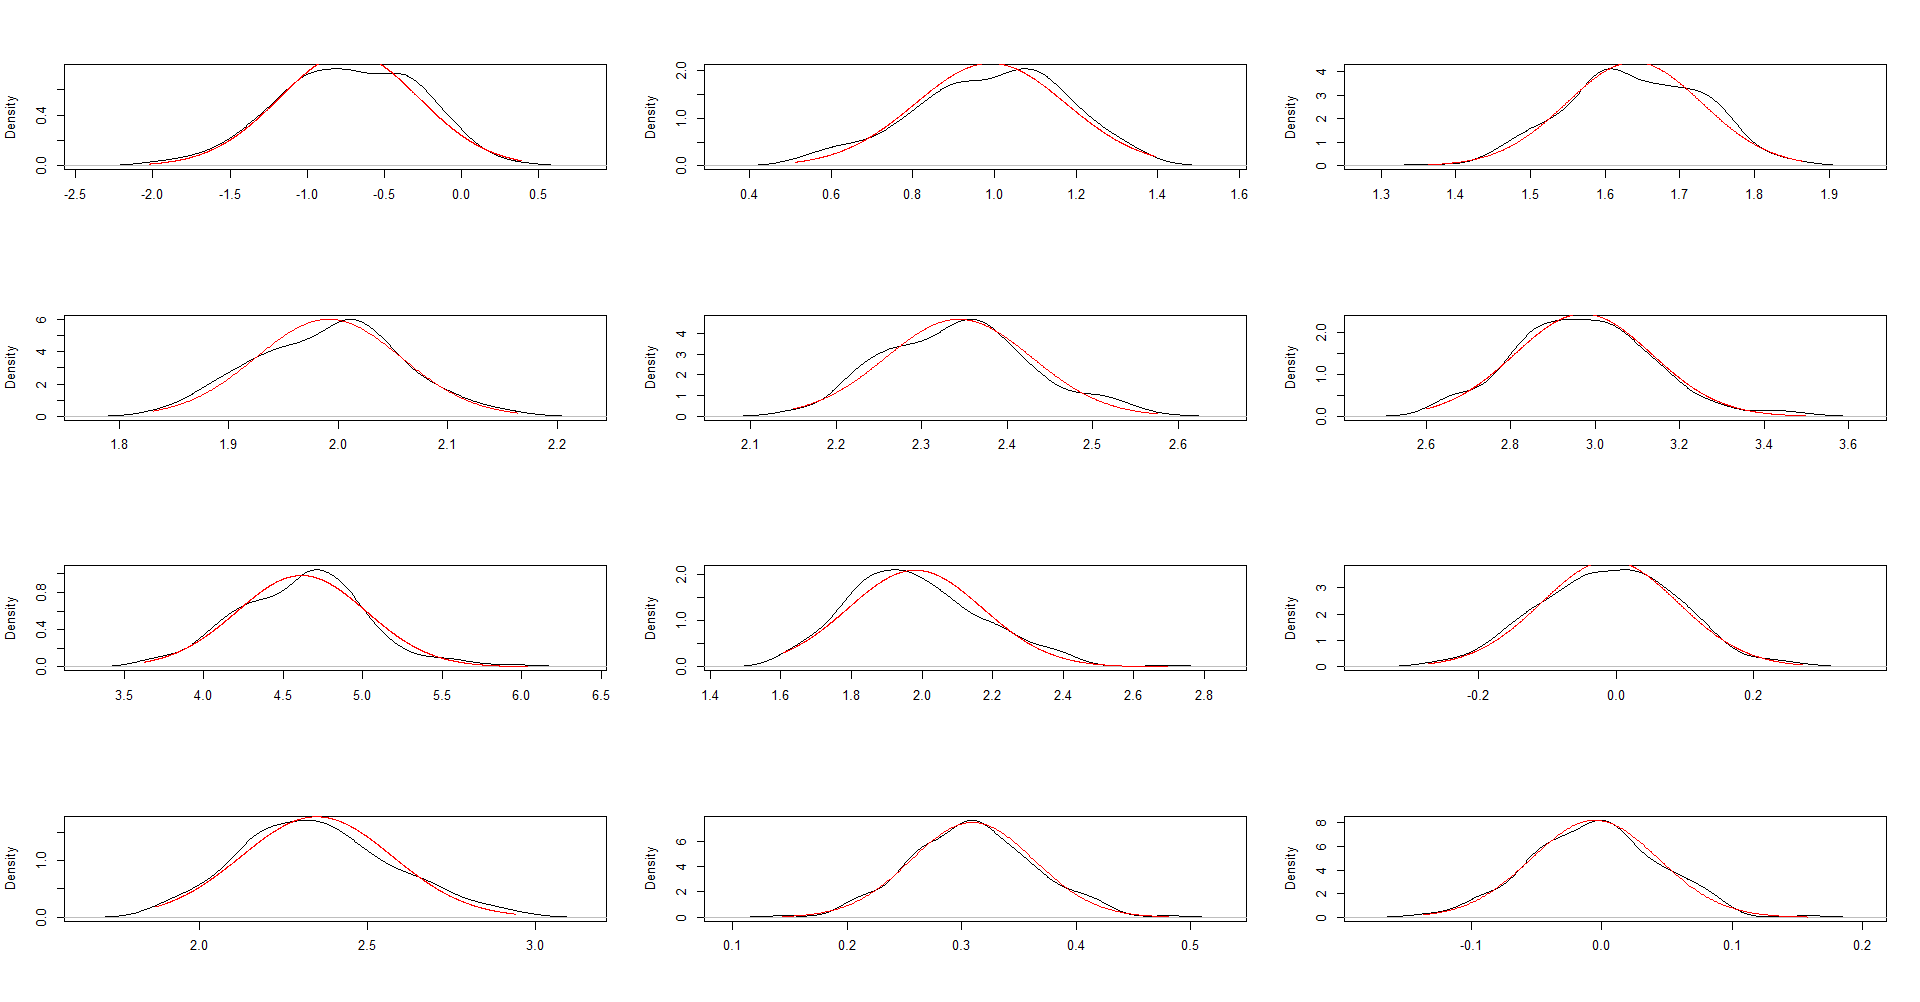
\includegraphics[width=340pt, height=200pt]{Chapters/chapter15/figures/DensitiesSum.png}
	\caption[List of figure caption goes here]{Density estimates of summary statistics: g-and-k simulation.}\label{figDensSum}
\end{figure} 

\begin{figure}[!h]
	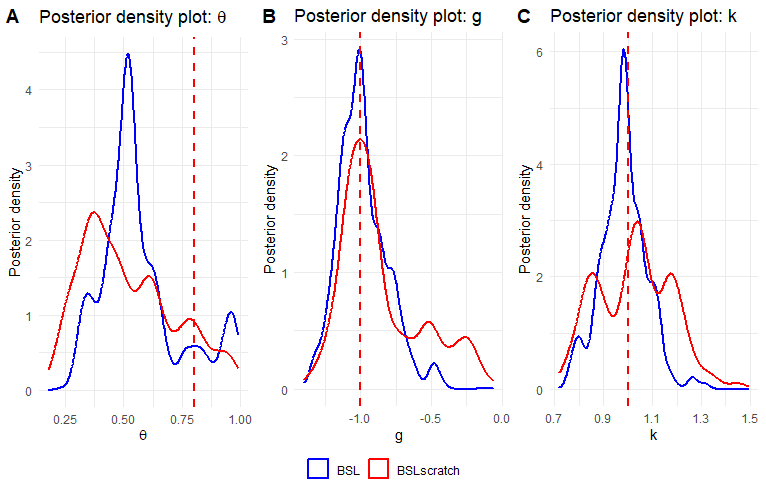
\includegraphics[width=340pt, height=200pt]{Chapters/chapter15/figures/BSLgksim.png}
	\caption[List of figure caption goes here]{Posterior distributions using Bayesian synthetic likelihood: g-and-k simulation.}\label{figBSL}
\end{figure}


\section{Optimization approaches}\label{sec15_2}

Traditional MCMC and importance sampling (IS) algorithms require pointwise evaluation of the likelihood function, which entails a massive number of operations when applied to very large datasets. Unfortunately, these algorithms are not designed to be \textit{scalable}, at least in their standard form (see Chapter~\ref{chap13} for alternatives). Moreover, when the parameter space is large, they also lack \textit{scalability} with respect to the number of parameters. Therefore, approximation methods should be considered even when the likelihood function has an analytical expression.

\textit{Optimization approaches} are designed to scale efficiently with high-dimensional parameter spaces and large datasets. The key idea is to replace simulation with optimization. In this section, we introduce the most common optimization approaches within the Bayesian inferential framework. 

\subsection{Integrated nested Laplace approximations}\label{sec15_21}
\textit{Integrated Nested Laplace Approximations} (INLA) is a deterministic approach for Bayesian inference in latent Gaussian models (LGMs) \cite{rue2009approximate}. In particular, INLA approximates the marginal posterior distributions using a combination of Laplace approximations, low-dimensional deterministic integration and optimization steps in sparse covariance settings \cite{rue2017bayesian}. The advantages of INLA compared to MCMC are that it is fast and does not suffer from poor mixing.

The point of departure is a structured additive regression model, where the response variable $y_i$ belongs to the exponential family such that the mean $\mu_i$ is linked to a linear predictor $\eta_i$ through the link function $g(\cdot)$, that is, $\eta_i=g(\mu_i)$, where
\begin{align*}
	\mu_i&=\alpha+\boldsymbol{\beta}^{\top}\boldsymbol{x}_{i}+\sum_{j=1}^{J}f^{(j)}(u_{ji})+\epsilon_{i},
\end{align*}
where $\alpha$ is the general intercept, $f^{(j)}$ are unknown functions of the covariates $\boldsymbol{u}_i$, $\boldsymbol{\beta}$ is a $K$-dimensional vector of linear effects associated with regressors $\boldsymbol{x}_i$, and $\epsilon_{i}$ is the unstructured error.

Note that latent Gaussian models encompass a wide range of relevant empirical models depending on the specific elements and structure involved in $f^{(j)}$, such as generalized linear models with unobserved heterogeneity, spatial and/or temporal dependence, and semi-parametric models.

Latent Gaussian models assign a Gaussian prior to $\alpha$, $\boldsymbol{\beta}$, $f^{(j)}$, and $(\epsilon_{i}$. Let $\boldsymbol{z}$ denote the vector of all latent Gaussian variables $\left\{\alpha, \boldsymbol{\beta}, f^{(j)},\eta_{i}\right\}$, where the dimension is potentially \( P = 1 + K + J + N \) (although this is not always the case), and let $\boldsymbol{\theta}$ be the $m$-dimensional vector of hyperparameters. Then, the density $\pi(\boldsymbol{z} \mid \boldsymbol{\theta}_1)$ is Gaussian with mean zero and precision matrix (i.e., the inverse of the covariance matrix) $\boldsymbol{Q}(\boldsymbol{\theta}_1)$.

The distribution of $\boldsymbol{y}$ is $p(\boldsymbol{y}\mid \boldsymbol{z},\boldsymbol{\theta}_2)$ such that $y_i$ are conditional independent given $z_i,\boldsymbol{\theta}_2$, $\boldsymbol{\theta}=[\boldsymbol{\theta}_1^{\top} \ \boldsymbol{\theta}_2^{\top}]^{\top}$, $i=1,2,\dots,N$. Thus, the posterior distribution is
\begin{align}\label{eq:INLA1}
	\pi(\boldsymbol{z},\boldsymbol{\theta}\mid \boldsymbol{y})&\propto \pi(\boldsymbol{\theta})\times \pi(\boldsymbol{z}\mid \boldsymbol{\theta}_1)\times \prod_{i=1}^{N}p(y_i\mid \boldsymbol{z},\boldsymbol{\theta}_2)\\
	&\propto \pi(\boldsymbol{\theta})|\boldsymbol{Q}(\boldsymbol{\theta}_1)|^{1/2}\exp\left\{-\frac{1}{2}\boldsymbol{z}^{\top}\boldsymbol{Q}(\boldsymbol{\theta}_1)\boldsymbol{z}+\sum_{i=1}^N\log p(y_i\mid z_i,\boldsymbol{\theta}_2)\right\}.\nonumber
\end{align}
Most models in INLA assume a conditional independence structure within the high-dimensional latent Gaussian field; that is, $\boldsymbol{z}$ is a Gaussian Markov random field (GMRF) with a sparse precision matrix $\boldsymbol{Q}(\boldsymbol{\theta}_1)$. A second key assumption is that the dimension of $\boldsymbol{\theta}$ is small, for instance, $m < 15$. These assumptions are essential for enabling fast approximate inference.

The main aim in INLA is to approximate the marginal posterior distributions $\pi(z_i\mid \boldsymbol{y})$ and $\pi(\theta_l\mid \boldsymbol{y})$, $l=1,2,\dots,m$.
The posterior distribution of $\boldsymbol{\theta}$ is
\begin{align*}	
	\pi(\boldsymbol{\theta}\mid \boldsymbol{y})&=\frac{p(\boldsymbol{y},\boldsymbol{\theta})}{p(\boldsymbol{y})}\\
	&=\frac{p(\boldsymbol{y},\boldsymbol{\theta})}{p(\boldsymbol{y})}\times \frac{\pi(\boldsymbol{z}\mid \boldsymbol{\theta},\boldsymbol{y})}{\pi(\boldsymbol{z}\mid\boldsymbol{\theta},\boldsymbol{y})}\\
	&=\frac{p(\boldsymbol{z},\boldsymbol{\theta},\boldsymbol{y})}{p(\boldsymbol{y})\pi(\boldsymbol{z}\mid \boldsymbol{\theta},\boldsymbol{y})}\\
	&\propto\frac{p(\boldsymbol{z},\boldsymbol{\theta},\boldsymbol{y})}{\pi(\boldsymbol{z}\mid \boldsymbol{\theta},\boldsymbol{y})}\\
	&\propto\frac{p(\boldsymbol{y}\mid \boldsymbol{z},\boldsymbol{\theta})\pi(\boldsymbol{z}\mid\boldsymbol{\theta})\pi(\boldsymbol{\theta})}{\pi(\boldsymbol{z}\mid \boldsymbol{\theta},\boldsymbol{y})}.
\end{align*}
The numerator in the previous expression is easy to calculate (see Equation~\ref{eq:INLA1}), but the denominator is generally not available in closed form and is difficult to compute. Thus, INLA approximates it at specific values $\boldsymbol{\theta}_g$,
\begin{align*}
	\pi_a(\boldsymbol{\theta}_g\mid \boldsymbol{y})&\propto\frac{p(\boldsymbol{y}\mid \boldsymbol{z},\boldsymbol{\theta}_g)\pi(\boldsymbol{z}\mid\boldsymbol{\theta}_g)\pi(\boldsymbol{\theta}_g)}{\pi_{a,G}(\boldsymbol{z}\mid \boldsymbol{\theta}_g,\boldsymbol{y})},
\end{align*} 
where $\pi_{a,G}(z_i \mid \boldsymbol{\theta}_g, \boldsymbol{y})$ is a Gaussian approximation that matches the mode and covariance matrix of the full posterior $\pi(\boldsymbol{z} \mid \boldsymbol{\theta}, \boldsymbol{y})$. 

The approximation error of $\pi_a(\boldsymbol{\theta} \mid \boldsymbol{y})$ is \( O(N^{-1}) \) under standard conditions, meaning that the error, when multiplied by \( N \), remains bounded \cite{Tierney1986, rue2009approximate}. However, in many applications using INLA, the dimension of the latent Gaussian variables, \( P \), increases with the sample size. In such cases, the error rate becomes \( O(P/N) \). When \( P/N \rightarrow 1 \), which occurs in many models, the approximation error becomes \( O(1) \): bounded, but potentially large.

Therefore, it is important to check the effective number of parameters, as the asymptotic error of $\pi_a(\boldsymbol{\theta} \mid \boldsymbol{y})$ depends on the dimension of $\boldsymbol{z}$. According to \cite{rue2009approximate}, in most of their applications the effective number of parameters is small relative to the sample size in regions near the mode of $\pi_a(\boldsymbol{\theta} \mid \boldsymbol{y})$. 

The marginal posterior $\pi(z_i \mid \boldsymbol{\theta}, \boldsymbol{y})$ is more challenging to compute due to the potentially high dimension of $\boldsymbol{z}$. It may seem intuitive to use the Gaussian approximation $\pi_{a,G}(\boldsymbol{z} \mid \boldsymbol{\theta}, \boldsymbol{y})$; however, this is often not sufficiently accurate due to its lack of skewness. An alternative is to use the following expression
\begin{align*}
	\pi(z_i\mid \boldsymbol{\theta},\boldsymbol{y})&=\frac{p(z_i,\boldsymbol{\theta},\boldsymbol{y})}{p(\boldsymbol{\theta},\boldsymbol{y})}\\
	&=\frac{p(z_i,\boldsymbol{\theta},\boldsymbol{y})}{p(\boldsymbol{\theta},\boldsymbol{y})}\times \frac{\pi(\boldsymbol{z}\mid\boldsymbol{\theta},\boldsymbol{y})}{\pi(\boldsymbol{z}\mid\boldsymbol{\theta},\boldsymbol{y})}\\
	&=\frac{\pi(\boldsymbol{z}\mid\boldsymbol{\theta},\boldsymbol{y})}{p(\boldsymbol{z},\boldsymbol{\theta},\boldsymbol{y})}\times p(z_i,\boldsymbol{\theta},\boldsymbol{y})\\
	&=\frac{\pi(\boldsymbol{z}\mid\boldsymbol{\theta},\boldsymbol{y})}{\pi(\boldsymbol{z}_{-i}\mid z_i,\boldsymbol{\theta},\boldsymbol{y})}\\
	&\propto \frac{p(\boldsymbol{y}\mid \boldsymbol{z},\boldsymbol{\theta})\pi(\boldsymbol{z}\mid\boldsymbol{\theta})\pi(\boldsymbol{\theta})}{\pi(\boldsymbol{z}_{-i}\mid z_i,\boldsymbol{\theta},\boldsymbol{y})}, 
\end{align*}
where the second-to-last equality follows from the identity $\pi(\boldsymbol{z}_{-i} \mid z_i, \boldsymbol{\theta}, \boldsymbol{y}) = \frac{p(\boldsymbol{z}, \boldsymbol{\theta}, \boldsymbol{y})}{p(z_i, \boldsymbol{\theta}, \boldsymbol{y})}$, $-i$ denotes all elements of $\boldsymbol{z}$ except the $i$-th, and approximating the denominator in the last expression using a simplified Laplace approximation, which corrects the Gaussian approximation for location and skewness via a Taylor series expansion about the mode of the Laplace approximation \cite{rue2009approximate}. This follows the spirit of the approximations developed by \cite{Tierney1986, tierney1989fully} for posterior moments and marginal densities, and is similar to those used in Chapter~\ref{chap10} when performing Bayesian model averaging (BMA) using the BIC information criterion. The discussion about the asymptotic error of the approximation $\pi_{a}(z_i \mid \boldsymbol{\theta}, \boldsymbol{y})$ follows the same arguments as those for $\pi_a(\boldsymbol{\theta} \mid \boldsymbol{y})$.

We can obtain the marginal posterior distributions integrating with respect to $\boldsymbol{\theta}$,
\begin{align*}
	\pi(z_i\mid \boldsymbol{y})&=\int_{{\Theta}} \pi(z_i\mid \boldsymbol{\theta},\boldsymbol{y})\pi(\boldsymbol{\theta}\mid\boldsymbol{y})d\boldsymbol{\theta}\\
	\pi(\theta_l\mid\boldsymbol{y})&=\int_{{\Theta}} \pi(\boldsymbol{\theta}\mid \boldsymbol{y})d\boldsymbol{\theta}_{-l}.
\end{align*}
This integrals are solve numerically using a smart grid around the mode of $\pi_a(\boldsymbol{\theta}\mid\boldsymbol{y})$. In particular, 
\begin{align*}
	\pi_a(z_i\mid \boldsymbol{y})&=\sum_{g=1}^G \pi_{a}(z_i\mid \boldsymbol{\theta}_g,\boldsymbol{y})\pi_a(\boldsymbol{\theta}_g\mid \boldsymbol{y})\Delta_g,
\end{align*}
where $\pi_{a}(z_i\mid \boldsymbol{\theta}_g,\boldsymbol{y})$ is the approximation of $\pi(z_i\mid \boldsymbol{\theta},\boldsymbol{y})$ evaluated at $\boldsymbol{\theta}_g$. Then, we have the sum over the values of $\boldsymbol{\theta}$ with area weights $\Delta_g$. If all support points are equidistant, then $\Delta_g = 1$.

Algorithm~\ref{INLA0} presents the INLA algorithm. Note that stages 2 and 3 correspond to the nested Laplace approximations, whereas stage 4 involves the integration step.
    
\begin{algorithm}
	\caption{Integrated nested Laplace approximations (INLA)}\label{INLA0}
	\begin{algorithmic}[1]
		\State Obtain the mode of $\pi_a(\boldsymbol{\theta}\mid \boldsymbol{y})$, that is $\boldsymbol{\theta}^*$, by maximizing $\log \pi_a(\boldsymbol{\theta}\mid \boldsymbol{y})$
		\State Compute $\pi_a(\boldsymbol{\theta}_g\mid \boldsymbol{y})$ for a set of high density points $\boldsymbol{\theta}_g$, $g=1,2,\dots,G$
		\State Compute the approximation $\pi_a(z_i\mid \boldsymbol{\theta}_g,\boldsymbol{y})$, $g=1,2,\dots,G$
		\State Compute $\pi_a(z_i\mid \boldsymbol{y})$ and $\pi_a(\theta_l\mid\boldsymbol{y})$ using numerical integration
		   
%		\State Obtain the covariance matrix of $\boldsymbol{\theta}$, that is, $\boldsymbol{\Sigma}$, as the negative inverse of the Hessian matrix of $\log \pi_a(\boldsymbol{\theta}\mid \boldsymbol{y})$
%		\State Perform the eigen value decomposition of $\boldsymbol{\Sigma}=\boldsymbol{V}\boldsymbol{\Lambda}\boldsymbol{V}^{\top}$, and defines $\boldsymbol{\theta}(\boldsymbol{e})=\boldsymbol{\theta}^*+\boldsymbol{V}\boldsymbol{\Lambda}^{1/2}\boldsymbol{e}$, where $\boldsymbol{e}\sim N(\boldsymbol{0},\boldsymbol{I}_m)$
%		\State Explore $\pi_a(\boldsymbol{\theta}\mid \boldsymbol{y})$ starting at $\boldsymbol{\theta}^*$ and step lengths $\delta_e=1$ in all up and down direction for each of the $m$ coordinates as long as $|\log \pi_a(\boldsymbol{\theta}(\boldsymbol{0})\mid \boldsymbol{y})-\log \pi_a(\boldsymbol{\theta}(\boldsymbol{e})\mid \boldsymbol{y})|<\delta_{\pi}$, where $\delta_{\pi}=2.5$. Note that this implies that $\Delta_l$ are equal
%		\State Use the previous explored points to interpolate and obtain an approximation $\pi_a(\boldsymbol{\theta}\mid \boldsymbol{y})$, and compute the marginals using numerical integration
%		\State Approximate $\pi(z_i\mid \boldsymbol{y})$ using Laplace approximations (see \cite{rue2009approximate} for details)       
	\end{algorithmic}
\end{algorithm}

Thus, INLA can be used in LGMs that satisfy \cite{rue2017bayesian,martino2019integrated}:
\begin{enumerate}
	\item There is conditional independence, that is, $y_i\perp y_s \mid \eta_i,\boldsymbol{\theta}$, such that $p(\boldsymbol{y}\mid \boldsymbol{z},\boldsymbol{\theta})=\prod_{i=1}^{N}p(y_i\mid \eta_i,\boldsymbol{\theta})$.
	\item The dimension of $\boldsymbol{\theta}$ is small, less than 15.
	\item $\boldsymbol{z}$ is a GMRF with sparse precision matrix.
	\item The linear predictor depends linearly on the smooth unknown functions of covariates.
	\item The inference is on the marginal posterior distributions $\pi(z_i\mid \boldsymbol{y})$ and $\pi(\theta_l\mid \boldsymbol{y})$.  
\end{enumerate} 

\cite{rue2009approximate} also discuss how to approximate the marginal likelihood and compute the deviance information criterion \cite{spiegelhalter2002bayesian} for model selection, as well as how to perform predictive analysis. 

The point of departure for INLA is the class of latent Gaussian models (LGMs); consequently, discrete latent classes are not supported. In addition, since INLA is based on approximations around the mode, it may struggle with models exhibiting multimodality, as there is no global exploration of the parameter space. 

Implementing INLA from scratch is a complex task \cite{martino2019integrated}; thus, applications are generally limited to the models implemented in the \texttt{INLA} package in \textbf{R}.\footnote{Visit https://www.r-inla.org/ for documentation.} However, there are new packages that implement specialized models, as well as recent developments that combine INLA with MCMC algorithms (see Table 2 in \cite{martino2019integrated} for details). 

%In particular, \cite{bivand2015spatial} developed the \textit{INLABMA} package to perform Bayesian model averaging (BMA) in spatial econometric models and MCMC-INLA. See also \cite{gomez2021estimating} for an application of INLA to spatial econometric models.\\

\textbf{Example: Poisson model with unobserved heterogeneity}

Let's simulate the model $Y_i \sim \text{Poisson}(\lambda_i)$, where $\lambda_i = \exp\left\{1 + x_i + \epsilon_i\right\}$, with $\epsilon_i \sim \mathcal{N}(0, 0.5^2)$ and $x_i \sim \mathcal{N}(0, 1^2)$ for $i = 1, 2, \dots, 10,\!000$. Note that $\epsilon_i$ represents the unobserved heterogeneity.

The following code demonstrates how to perform inference on this model using the \textit{INLA} package. Keep in mind that INLA specifies Gaussian priors in terms of precision, which is the inverse of the variance.

We present the results obtained using the three approximation strategies available in INLA: Simplified Laplace (default), Gaussian, and full Laplace. In this example, the results are practically identical across methods (see Figures~\ref{FigINLA1} and~\ref{FigINLA2}), and all 95\% credible intervals contain the true population parameters. Despite the large sample size, INLA performs inference in a matter of seconds.

\begin{tcolorbox}[enhanced,width=4.67in,center upper,
	fontupper=\large\bfseries,drop shadow southwest,sharp corners]
	\textit{R code. Integrated Nested Laplace Approximations: Poisson model with unobserved heterogeneity}
	\begin{VF}
		\begin{lstlisting}[language=R]
# Install Rtools according to your R version
# Check Rtolls is properly installed
# Install INLA
# install.packages("INLA",repos=c(getOption("repos"),INLA="https://inla.r-inla-download.org/R/stable"), dep=TRUE)
rm(list = ls()); set.seed(010101); library(INLA)
n <- 10000; x <- rnorm(n, sd = 1); u <- rnorm(n, sd = 0.5)
intercept <- 1; beta <- 1; id <- 1:n
y <- rpois(n, lambda = exp(intercept + beta * x + u))
my.data <- data.frame(y, x, id)
formula <- y ~ 1 + x + f(id, model="iid")
inla.sla <- inla(formula, data = my.data, family = "poisson", control.compute=list(return.marginals.predictor=TRUE))
inla.ga <- inla(formula, data = my.data, family = "poisson", control.inla = list(strategy = "gaussian", int.strategy = "eb"), control.compute=list(return.marginals.predictor=TRUE))
inla.la <- inla(formula, data = my.data, family = "poisson", control.inla = list(strategy = "laplace", int.strategy = "grid", dz=0.1, diff.logdens=20),
control.compute=list(return.marginals.predictor=TRUE))
summary(inla.sla)
marg_sla <- inla.sla$marginals.fixed$x
marg_ga  <- inla.ga$marginals.fixed$x
marg_la  <- inla.la$marginals.fixed$x
plot(marg_sla, type = "l", col = "blue", lwd = 2, xlab = expression(beta[x]), ylab = "Density", main = "Posterior of slope under different INLA strategies")
lines(marg_ga, col = "green", lwd = 2, lty = 2)
lines(marg_la, col = "red", lwd = 2, lty = 3)
abline(v = 1, col = "black", lty = 4, lwd = 2)
legend("topright", legend = c("Simplified Laplace", "Gaussian", "Full Laplace", "True = 1"), col = c("blue", "green", "red", "black"), lwd = 2, lty = c(1, 2, 3, 4), bty = "n")
# Summary beta sla
inla.qmarginal(c(0.025, 0.5, 0.975), marg_sla) # 95% credible interval
# Variance
marg.prec.sla <- inla.sla$marginals.hyperpar[["Precision for id"]]
marg.prec.ga  <- inla.ga$marginals.hyperpar[["Precision for id"]]
marg.prec.la  <- inla.la$marginals.hyperpar[["Precision for id"]]
marg.var.sla <- inla.tmarginal(function(x) 1/x, marg.prec.sla)
marg.var.ga  <- inla.tmarginal(function(x) 1/x, marg.prec.ga)
marg.var.la  <- inla.tmarginal(function(x) 1/x, marg.prec.la)
\end{lstlisting}
	\end{VF}
\end{tcolorbox}

\begin{tcolorbox}[enhanced,width=4.67in,center upper,
	fontupper=\large\bfseries,drop shadow southwest,sharp corners]
	\textit{R code. Integrated Nested Laplace Approximations: Poisson model with unobserved heterogeneity}
	\begin{VF}
		\begin{lstlisting}[language=R]
# Base plot
plot(marg.var.sla, type = "l", col = "blue", lwd = 2, xlab = expression(sigma^2), ylab = "Density", main = "Posterior of Random Effect Variance")
lines(marg.var.ga, col = "green", lwd = 2, lty = 2)
lines(marg.var.la, col = "red", lwd = 2, lty = 3)
abline(v = 0.25, col = "black", lty = 4, lwd = 2)
legend("topright", legend = c("Simplified Laplace", "Gaussian", "Full Laplace", "True Variance (0.25)"), col = c("blue", "green", "red", "black"), lwd = 2, lty = c(1, 2, 3, 4), bty = "n")
# Summary variance sla
inla.qmarginal(c(0.025, 0.5, 0.975), marg.var.sla) # 95% credible interval
\end{lstlisting}
	\end{VF}
\end{tcolorbox}

\begin{figure}[!h]
	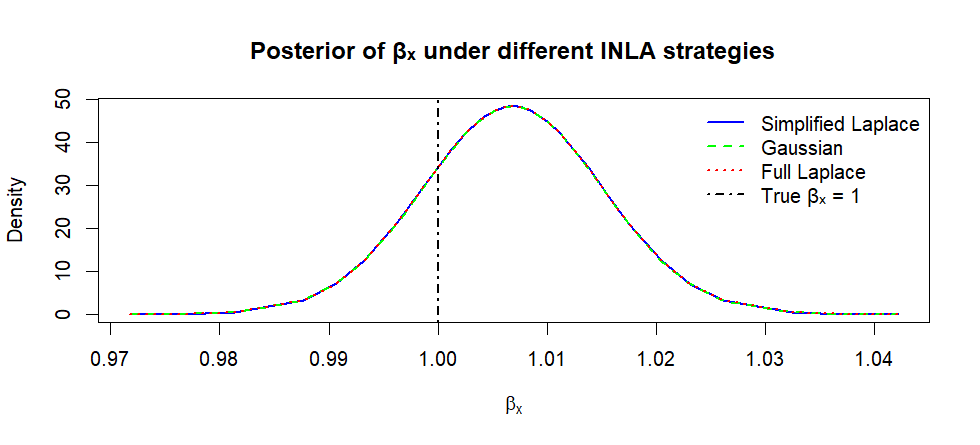
\includegraphics[width=340pt, height=200pt]{Chapters/chapter15/figures/FigINLA1.png}
	\caption[List of figure caption goes here]{Density estimates of slope parameter: Three approximations in INLA.}\label{FigINLA1}
\end{figure} 

\begin{figure}[!h]
	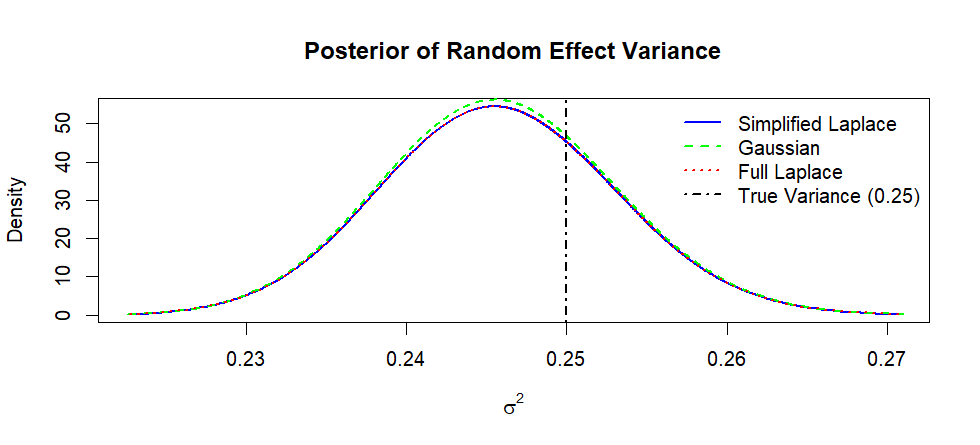
\includegraphics[width=340pt, height=200pt]{Chapters/chapter15/figures/FigINLA2.png}
	\caption[List of figure caption goes here]{Density estimates of variance: Three approximations in INLA.}\label{FigINLA2}
\end{figure} 

\textbf{Example: Spatial econometrics model}

The starting point of spatial econometrics is the \textit{contiguity} or \textit{adjacency} matrix \( W \), which defines which spatial polygons (regions) are considered neighbors. This is an \( N \times N \) matrix, where each row and column corresponds to a spatial polygon, and a non-zero element indicates that two polygons are neighbors. By construction, the main diagonal is equal to zero, meaning that no polygon is a neighbor to itself. Given its structure, the contiguity matrix is sparse.

There are various ways to define contiguity between spatial units, with two of the most commonly used criteria being the \textit{queen} and \textit{rook} criteria, inspired by chess. In the queen criterion, two spatial units are considered neighbors if they share any part of a boundary or a point. In contrast, under the rook criterion, two units are considered neighbors only if they share a common boundary edge; they must touch along at least one side, and corner contact is not sufficient to establish a neighbor relationship.

However, users may apply any contiguity criteria they deem appropriate, depending on the context. For example, contiguity can be defined based on factors like the travel time by car between centroids or the proximity of main towns between municipalities. Typically, the contiguity matrix \( W \) is binary, with a value of 1 indicating that two regions are neighbors and 0 otherwise. Additionally, contiguity matrices are often row-standardized to facilitate the analysis of spatial stationarity.

\cite{lesage2009introduction,bivand2015spatial} present the most commonly used specifications in spatial econometrics, namely the spatial error model (SEM), the spatial autoregressive model (SAR), and the spatial Durbin model (SDM), which can, in turn, be combined to form the general nesting spatial (GNS) model \cite{elhorst2014spatial,Ramirez2017}. In particular, the SEM sets
\begin{align*}
	\boldsymbol{y} &= \boldsymbol{X\beta} + \boldsymbol{\mu}\\
	\boldsymbol{\mu} &= \lambda\boldsymbol{W\mu} + \boldsymbol{\epsilon},
\end{align*}
where $\boldsymbol{\epsilon}\sim N(\boldsymbol{0}_N,\sigma^2\boldsymbol{I}_N)$. Then, $\boldsymbol{\mu}=(\boldsymbol{I}_N-\rho\boldsymbol{W})^{-1}\boldsymbol{\epsilon}$, which implies that 
\begin{align*}
	\boldsymbol{y} &= \boldsymbol{X\beta} + \boldsymbol{e},
\end{align*}
where $\boldsymbol{e}\sim N(\boldsymbol{0},\sigma^2(\boldsymbol{I}_N-\rho\boldsymbol{W})^{-1}(\boldsymbol{I}_N-\rho\boldsymbol{W}^{\top})^{-1})$. In this model $\lambda$ controls the degree of spatial dependence. 

The SAR sets
\begin{align*}
	\boldsymbol{y} &= \rho\boldsymbol{Wy} + \boldsymbol{X\beta} + \boldsymbol{\mu}\\
	 &= (\boldsymbol{I}_N-\rho\boldsymbol{W})^{-1}\boldsymbol{X\beta} + \boldsymbol{\epsilon},
\end{align*}
where $\boldsymbol{\epsilon}=(\boldsymbol{I}_N-\rho\boldsymbol{W})^{-1}\boldsymbol{\mu}$.

The SDM sets
\begin{align*}
	\boldsymbol{y} &= \rho\boldsymbol{Wy} + \boldsymbol{X\beta} +  \boldsymbol{WX\delta} + \boldsymbol{\mu}\\
	&= (\boldsymbol{I}_N-\rho\boldsymbol{W})^{-1}(\boldsymbol{X\beta} +  \boldsymbol{WX\delta}) + \boldsymbol{\epsilon},
\end{align*}
where $\boldsymbol{\epsilon}=(\boldsymbol{I}_N-\rho\boldsymbol{W})^{-1}\boldsymbol{\mu}$.

The degree of spatial dependence in the SAR and SDM models is determined by the parameter \( \rho \). Note that the SDM model is similar to the SAR model, except that it also includes spatial lags of the regressors as additional covariates.

\cite{ord75} and \cite{anselin82} show that a necessary condition for weak stationarity in spatial autoregressive processes with a row-standardized contiguity matrix is that the spatial autocorrelation coefficient must lie between \( 1/\omega_{\min} \) and 1, where \( \omega_{\min} \) is the smallest (most negative) eigenvalue of the contiguity matrix.\footnote{This is a necessary condition to ensure weak stationarity but is not sufficient due to edge and corner effects \cite[]{haining90}.}

Note that these three models, conditional on the spatial parameter, are standard linear regressions, which can be easily estimated using \textit{INLA}. \cite{bivand2015spatial} use the \textit{INLABMA} package to estimate these models conditional on different values of the spatial parameters, and then perform Bayesian Model Averaging (BMA) using the resulting estimates. In particular, it is necessary to define a grid over the spatial parameters, perform Bayesian inference using INLA for each value in the grid, and then aggregate the posterior results using BMA.

We now perform Bayesian inference on a spatial econometric model using the \textit{INLA} and \textit{INLABMA} packages, based on the dataset provided by \cite{ramirez2019welfare}, who conducted a Bayesian analysis of electricity demand in the department of Antioquia (Colombia), accounting for spatial dependence between municipalities in the region using a Conditional Autoregressive (CAR) spatial model. In particular, we conduct inference using the following specification:
\begin{align*}
	\log(\text{Electricity}_i)&=\beta_1+\beta_2\log(\text{Elect. price}_i)+\beta_3\log(\text{Income}_i)\\
	&+\beta_4\log(\text{Subs. price}_i)+\mu_i,
\end{align*} 
where \( \boldsymbol{\mu} = \lambda \boldsymbol{W} \boldsymbol{\mu} + \epsilon \); \textit{Electricity} is the average per capita annual consumption of electricity by individuals living in households of stratum one in each municipality of the department of Antioquia; \textit{Elect. price} is the average price of electricity (per kWh); \textit{Income} is the average per capita annual income; and \textit{Subs. price} is the average price of an electricity substitute (see \cite{ramirez2019welfare} for details).

The following code illustrates how to carry out a spatial econometric analysis. First, we download the files needed to plot the maps and construct the contiguity matrix. These files are available in the folder \textit{DataApp/Antioquia} of our GitHub repository: \textbf{https://github.com/besmarter/BSTApp}. The initial part of the code demonstrates how to download the \textit{GitHub} repository and extract the necessary files for mapping.

Figure~\ref{FigINLAmap1} displays the average electricity consumption per municipality. We observe the presence of spatial clusters, particularly in the northwestern region, which corresponds to a low-altitude area along the Caribbean coast.

The second part of the code constructs the contiguity matrix using the queen criterion. Figure~\ref{FigINLAmap2} illustrates the spatial links between municipalities. Following this, we estimate a standard Ordinary Least Squares (OLS) regression and conduct spatial autocorrelation tests on the residuals. The null hypothesis of both the global and local Moran's I tests is the absence of spatial autocorrelation in the OLS residuals. We reject the null hypothesis.

Finally, we perform Bayesian inference over a predefined grid of values for the spatial coefficient and apply Bayesian Model Averaging (BMA) using the \textit{INLABMA} package. Figure~\ref{FigINLArho} shows the BMA posterior distribution of the spatial coefficient in the SEM, which indicates the presence of spatial dependence. Figure~\ref{FigINLApriceelast} displays the posterior density of the own-price elasticity of electricity demand.
   
\begin{tcolorbox}[enhanced,width=4.67in,center upper,
	fontupper=\large\bfseries,drop shadow southwest,sharp corners]
	\textit{R code. Spatial econometric analysis: Spatial error model using INLA}
	\begin{VF}
		\begin{lstlisting}[language=R]
rm(list = ls()); set.seed(010101)
library(sf); library(tmap); library(classInt)
library(RColorBrewer); library(spdep); library(parallel)
library(INLABMA); library(sf); library(INLA)
zip_url <- "https://github.com/BEsmarter-consultancy/BSTApp/archive/refs/heads/master.zip"
temp_zip <- tempfile(fileext = ".zip")
download.file(zip_url, temp_zip, mode = "wb")
temp_dir <- tempdir()
unzip(temp_zip, exdir = temp_dir)
antioquia_path <- file.path(temp_dir, "BSTApp-master", "DataApp", "Antioquia")
list.files(antioquia_path)
antioquia_path <- file.path(temp_dir, "BSTApp-master", "DataApp", "Antioquia")
shp_file <- file.path(antioquia_path, "Antioquia.shp")
antioquia <- st_read(shp_file)
print(antioquia)
plot(st_geometry(antioquia), main = "Map of Antioquia")
interval <- classIntervals(antioquia$CONS_OLD, 5, style = "quantile")
antioquia$cons_class <- cut(antioquia$CONS_OLD,breaks = interval$brks,include.lowest = TRUE)
plotcolors <- brewer.pal(5, "Reds")
tmap_mode("plot")
tm_shape(antioquia) +
tm_fill(fill = "cons_class", fill.scale = tm_scale(values = plotcolors), fill.legend = tm_legend(title = "Electricity consumption")) + tm_borders(col = "grey90") + tm_compass(type = "8star", position = c("right", "top")) + tm_layout(legend.outside = TRUE)
nb_object <- poly2nb(antioquia, queen = TRUE)
centroids <- st_centroid(st_geometry(antioquia))
coords <- st_coordinates(centroids)
plot(st_geometry(antioquia), border = "grey")
plot(nb_object, coords, add = TRUE, col = "red")
attach(antioquia)
fform <- L_CONS_OLD ~ L_P_OLD + L_ING_US + L_P_SUST 
RegOLS <- lm(fform)
summary(RegOLS)
res <- RegOLS$residuals
NBList <- nb2listw(nb_object, style = "B")
moran_mc<- moran.mc(res, listw = NBList, 10000)
LM<-localmoran(as.vector(res), NBList)
sum(LM[,5]<0.05)
# Bayesian estimation
zero.variance <- list(prec = list(initial = 25, fixed = TRUE))
ant.mat <- nb2mat(nb_object)
bmsp <- as(ant.mat, "CsparseMatrix")
antioquia$idx <- 1:nrow(antioquia)
rrho1 <- seq(0.5, 0.95, len = 10)
\end{lstlisting}
	\end{VF}
\end{tcolorbox}

\begin{tcolorbox}[enhanced,width=4.67in,center upper,
	fontupper=\large\bfseries,drop shadow southwest,sharp corners]
	\textit{R code. Spatial econometric analysis: Spatial error model using INLA}
	\begin{VF}
		\begin{lstlisting}[language=R]
semmodels <- mclapply(rrho1, function(rho) {
	sem.inla(fform, d = as.data.frame(antioquia), W = bmsp, rho = rho,
	family = "gaussian", impacts = FALSE,
	control.family = list(hyper = zero.variance),
	control.predictor = list(compute = TRUE),
	control.compute = list(dic = TRUE, cpo = TRUE),
	control.inla = list(print.joint.hyper = TRUE))
})
bmasem <- INLABMA(semmodels, rrho1, 0, impacts = FALSE)
#Display results
plot(bmasem$rho$marginal, type="l", col = "blue", lwd = 2, xlab = expression(lambda), ylab = "Density", main = "Spatial error model: Posterior spatial coefficient")
bmasem[["rho"]][["quantiles"]]
marg_sla <- bmasem[["marginals.fixed"]][["L_P_OLD"]]
plot(marg_sla, type = "l", col = "blue", lwd = 2, xlab = expression(beta[x]), ylab = "Density", main = "Spatial error model: Posterior price elasticity")
bmasem[["summary.fixed"]]
\end{lstlisting}
	\end{VF}
\end{tcolorbox}

\begin{figure}[!h]
	\centering
	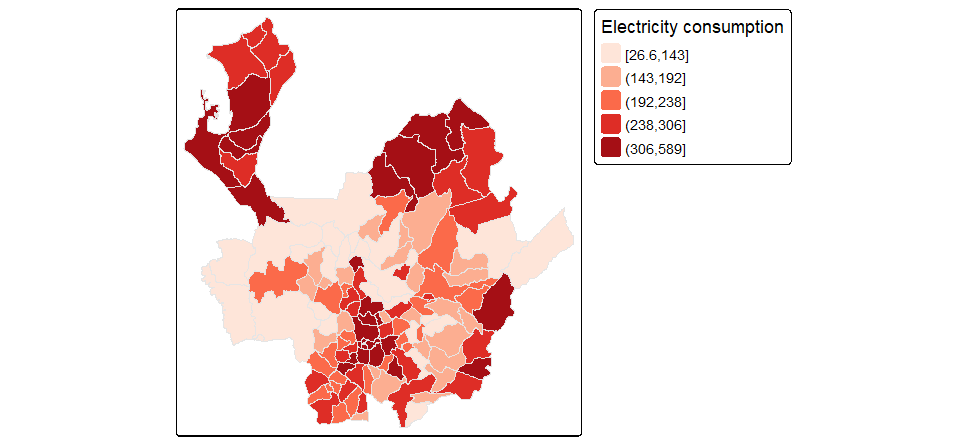
\includegraphics[width=340pt]{Chapters/chapter15/figures/AntMap.png}
	\caption[List of figure caption goes here]{Per capita annual average electricity consumption: Stratum 1, Antioquia (Colombia).}
	\label{FigINLAmap1}
\end{figure}

\begin{figure}[!h]
	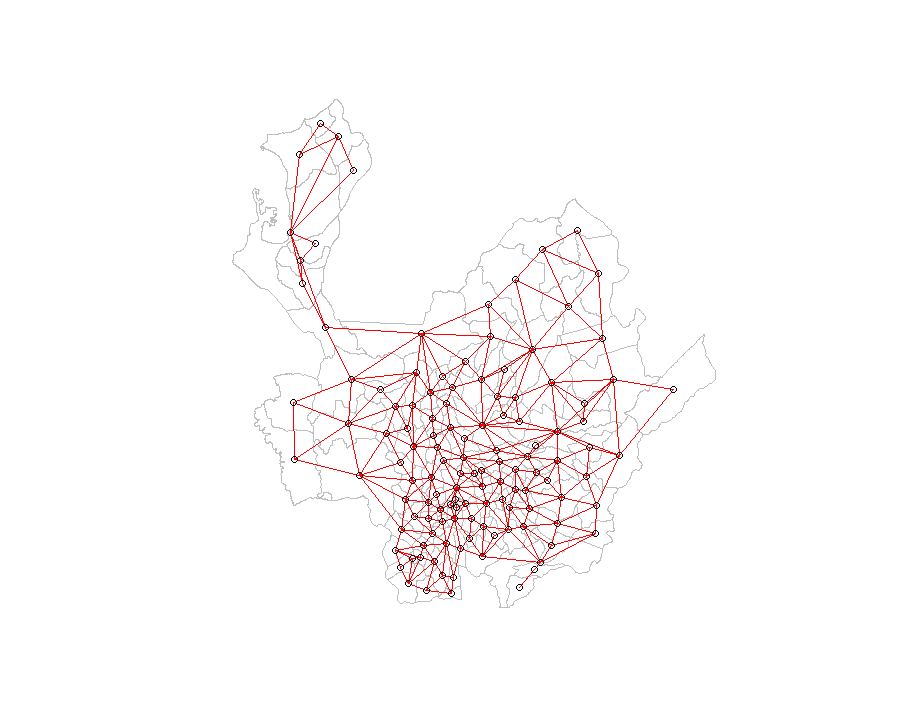
\includegraphics[width=340pt]{Chapters/chapter15/figures/AntMapCont.png}
	\caption[List of figure caption goes here]{Contiguity map: Queen criterion, municipalities (Antioquia, Colombia).}\label{FigINLAmap2}
\end{figure} 

\begin{figure}[!h]
	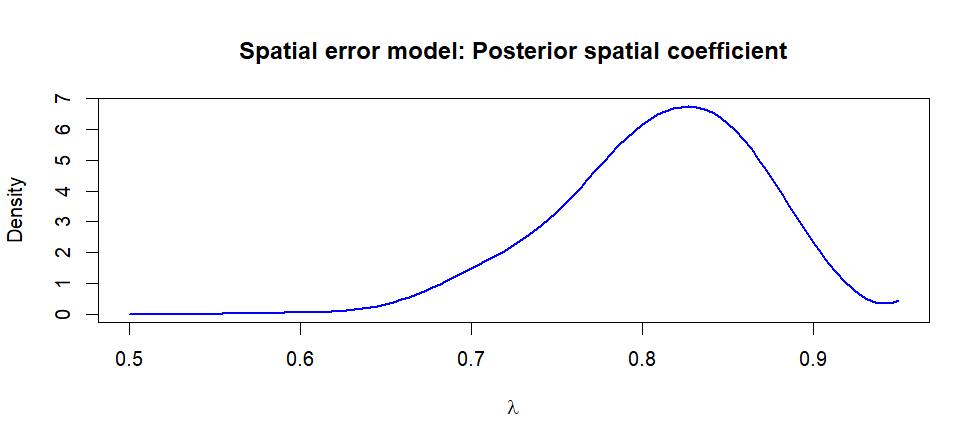
\includegraphics[width=340pt]{Chapters/chapter15/figures/SpaCoeff.png}
	\caption[List of figure caption goes here]{BMA posterior density: Spatial error coefficient.}\label{FigINLArho}
\end{figure} 

\begin{figure}[!h]
	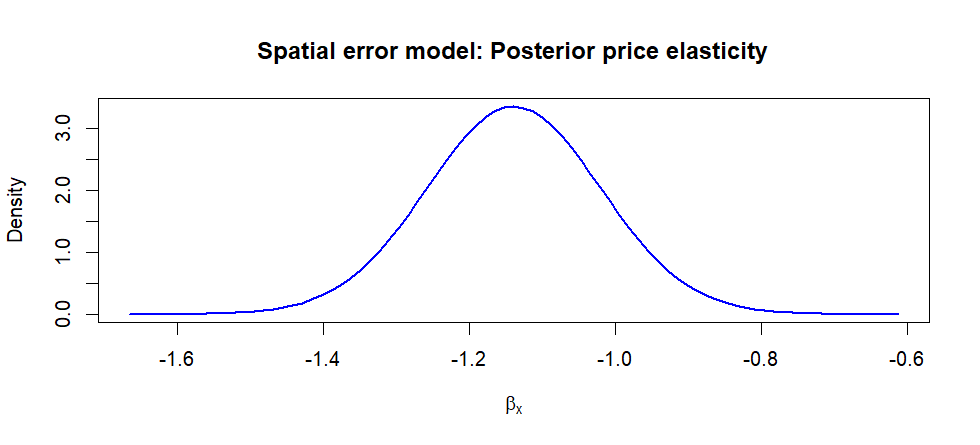
\includegraphics[width=340pt]{Chapters/chapter15/figures/PriceElast.png}
	\caption[List of figure caption goes here]{BMA posterior density: Own-price elasticity of electricity.}\label{FigINLApriceelast}
\end{figure} 


\subsection{Variational Bayes}\label{sec15_22}
\textit{Variational Bayes} (VB) is a method from machine learning \cite{jordan1999introduction, wainwright2008graphical} that replaces $\pi(\boldsymbol{\theta} \mid \mathbf{y})$ with an approximation obtained through optimization using the calculus of variations, hence the name \textit{variational} Bayes. This approach is useful when the posterior distribution is complex (e.g., multimodal) or when the parameter space is high-dimensional, making MCMC or IS algorithms computationally expensive.

The goal in VB is to approximate the posterior distribution using a distribution $q(\boldsymbol{\theta})$ from a variational family $\mathcal{Q}$ —a class of distributions that is computationally convenient yet flexible enough to closely approximate the true posterior \cite{blei2017variational}-. The distribution $q$ is called the \textit{variational approximation} to the posterior, and a particular $q$ in $\mathcal{Q}$ is defined by a specific set of \textit{variational parameters}. Typically, this approximation is obtained by minimizing the Kullback–Leibler (KL) divergence between $q(\boldsymbol{\theta})$ and $\pi(\boldsymbol{\theta} \mid \mathbf{y})$.
\begin{align}\label{eq:VB1}
	q^*(\boldsymbol{\theta}):=\underset{q \in \mathcal{Q}}{\argmin} \  \text{KL}(q(\boldsymbol{\theta})||\pi(\boldsymbol{\theta} \mid \mathbf{y})),
\end{align}  
where $\text{KL}(q(\boldsymbol{\theta}) \| \pi(\boldsymbol{\theta} \mid \mathbf{y})) = \mathbb{E}_q\left[\log\left(\frac{q(\boldsymbol{\theta})}{\pi(\boldsymbol{\theta} \mid \mathbf{y})}\right)\right]$.\footnote{The Kullback–Leibler (KL) divergence, also known as relative entropy, is non-negative: it equals 0 when $q(\boldsymbol{\theta}) = \pi(\boldsymbol{\theta} \mid \mathbf{y})$, and is positive otherwise. However, it does not satisfy the triangle inequality and is not symmetric, that is, $\text{KL}(q(\boldsymbol{\theta}) \| \pi(\boldsymbol{\theta} \mid \mathbf{y})) \neq \text{KL}(\pi(\boldsymbol{\theta} \mid \mathbf{y}) \| q(\boldsymbol{\theta}))$. Therefore, it is not a true distance (metric).}

Note that in relatively complex models, the optimization in Equation~\ref{eq:VB1} is not computable because it depends on the marginal likelihood $p(\boldsymbol{y})$, which is typically unknown due to the intractability of the integral involved. However, there is a solution to this problem. Let’s see:
\begin{align*}
	\log(p(\boldsymbol{y}))&=\log\left(\int_{\boldsymbol{\Theta}}p(\boldsymbol{y}\mid \boldsymbol{\theta})\pi(\boldsymbol{\theta})d\boldsymbol{\theta}\right)\\
	&=\log\left(\int_{\boldsymbol{\Theta}}p(\boldsymbol{y}, \boldsymbol{\theta})d\boldsymbol{\theta}\right)\\
	&=\log\left(\int_{\boldsymbol{\Theta}}\frac{p(\boldsymbol{y}, \boldsymbol{\theta})}{q(\boldsymbol{\theta})}q(\boldsymbol{\theta})d\boldsymbol{\theta}\right)\\
	&=\log \mathbb{E}_q\left(\frac{p(\boldsymbol{y}, \boldsymbol{\theta})}{q(\boldsymbol{\theta})}\right)\\
	&\geq \mathbb{E}_q\log\left(\frac{p(\boldsymbol{y}, \boldsymbol{\theta})}{q(\boldsymbol{\theta})}\right)\\
	&=\mathbb{E}_q\log(p(\boldsymbol{y}, \boldsymbol{\theta}))-\mathbb{E}_q\log(q(\boldsymbol{\theta}))\\
	&=\text{ELBO}(q(\boldsymbol{\theta})),
\end{align*}
where the inequality follows from Jensen's inequality, since $\log(\cdot)$ is concave. The last term is the \textit{evidence lower bound} (ELBO), which serves as a lower bound for the marginal likelihood. Note that the gap between the marginal likelihood and the ELBO is given by
\begin{align*}
	\log(p(\boldsymbol{y})) - \text{ELBO}(q(\boldsymbol{\theta})) & = \log(p(\boldsymbol{y})) - \mathbb{E}_q\log(p(\boldsymbol{y}, \boldsymbol{\theta}))+\mathbb{E}_q\log(q(\boldsymbol{\theta}))\\
	&=\mathbb{E}_q\left(\log(q(\boldsymbol{\theta}))-\log\left(\frac{p(\boldsymbol{y}, \boldsymbol{\theta})}{p(\boldsymbol{y})}\right)\right)\\
	&=\mathbb{E}_q\left(\log(q(\boldsymbol{\theta}))-\log\left(\frac{p(\boldsymbol{y}\mid \boldsymbol{\theta})\pi( \boldsymbol{\theta})}{p(\boldsymbol{y})}\right)\right)\\
	&=\mathbb{E}_q\left(\log(q(\boldsymbol{\theta}))-\log(\pi(\boldsymbol{\theta}\mid \boldsymbol{y}))\right)\\
	&=\text{KL}(q(\boldsymbol{\theta})||\pi(\boldsymbol{\theta} \mid \mathbf{y})).	 
\end{align*}
Then,
\begin{align*}
	\log(p(\boldsymbol{y})) = \text{KL}(q(\boldsymbol{\theta})||\pi(\boldsymbol{\theta} \mid \mathbf{y})) + \text{ELBO}(q(\boldsymbol{\theta})),  
\end{align*} 
which implies that maximizing the ELBO with respect to $q(\boldsymbol{\theta})$ is equivalent to minimizing the KL divergence, since $\log(p(\boldsymbol{y}))$ does not depend on $q(\boldsymbol{\theta})$. This avoids the need to compute the marginal likelihood and, consequently, makes the variational problem easier to solve. In addition, it provides a lower bound for the marginal likelihood, which can potentially be used for model selection. Thus, solving problem \ref{eq:VB1} is equivalent to solving
\begin{align}\label{eq:VB2}
	q^*(\boldsymbol{\theta}):=\underset{q \in \mathcal{Q}}{\argmax} \  \text{ELBO}(q(\boldsymbol{\theta})).
\end{align}

Note that the ELBO can be also expressed as 
\begin{align*}
	\text{ELBO}(q(\boldsymbol{\theta}))&=\mathbb{E}_q\log(p(\boldsymbol{y}, \boldsymbol{\theta}))-\mathbb{E}_q\log(q(\boldsymbol{\theta}))\\
	&=\mathbb{E}_q\log(p(\boldsymbol{y}\mid \boldsymbol{\theta}))+\mathbb{E}_q\log(\pi(\boldsymbol{\theta}))-\mathbb{E}_q\log(q(\boldsymbol{\theta}))\\
	&=\mathbb{E}_q\log(p(\boldsymbol{y}\mid \boldsymbol{\theta}))-\text{KL}(q(\boldsymbol{\theta})||\pi(\boldsymbol{\theta})).
\end{align*} 
This means that when maximizing the ELBO, we seek the distribution $q(\boldsymbol{\theta})$ that both maximizes the likelihood and minimizes the KL divergence between the variational distribution and the prior. In other words, we aim to strike a balance between the prior and the likelihood, which aligns with the core principle of Bayesian inference deriving the posterior distribution.

The most common approach for specifying $q(\boldsymbol{\theta})$ is to assume independence across blocks of $\boldsymbol{\theta}$, i.e., $q(\boldsymbol{\theta}) = \prod_{l=1}^K q_l(\boldsymbol{\theta}_l)$. This is known as the \textit{mean-field variational family}, a term that originates from statistical physics. Each $q_l(\boldsymbol{\theta}_l)$ is parameterized by a set of \textit{variational parameters}, and optimization is performed with respect to these parameters. Note that the mean-field approximation does not capture dependencies between parameters, although it can approximate the marginal distributions.

Let us now decompose the ELBO under the mean-field variational family \cite{nguyen2023depth},
\begin{align*}
		\text{ELBO}(q(\boldsymbol{\theta}))&=\mathbb{E}_q\log(p(\boldsymbol{y}, \boldsymbol{\theta}))-\mathbb{E}_q\log(q(\boldsymbol{\theta}))\\
	&=\int_{\mathbb{R}^K} \log(p(\boldsymbol{y}, \boldsymbol{\theta}))q(\boldsymbol{\theta})d\boldsymbol{\theta}-\int_{\mathbb{R}^K}\log(q(\boldsymbol{\theta}))q(\boldsymbol{\theta})d\boldsymbol{\theta}\\
	&=\int_{\mathbb{R}^K} \log\left(p(\boldsymbol{y}, \boldsymbol{\theta})\right)\prod_{l=1}^K q_l(\boldsymbol{\theta}_l)d\boldsymbol{\theta}_l-\int_{\mathbb{R}^K}\log\left(\prod_{l=1}^K q_l(\boldsymbol{\theta}_l)\right)\prod_{l=1}^K q_l(\boldsymbol{\theta}_l)d\boldsymbol{\theta}_l\\
	&=\int_{\mathbb{R}} \underbrace{\left(\int_{\mathbb{R}^{K-1}}\log\left(p(\boldsymbol{y}, \boldsymbol{\theta})\right)\prod_{l\neq k} q_l(\boldsymbol{\theta}_l)d\boldsymbol{\theta}_l\right)}_{\mathbb{E}_{-k}(\log\left(p(\boldsymbol{y}, \boldsymbol{\theta})\right))}q_k(\boldsymbol{\theta}_k)d\boldsymbol{\theta}_k\\ 
	&-\int_{\mathbb{R}}\log(q_k(\boldsymbol{\theta}_k))q_k(\boldsymbol{\theta}_k)d\boldsymbol{\theta}_k-\sum_{l\neq k}\int_{\mathbb{R}}\log(q_l(\boldsymbol{\theta}_l))q_l(\boldsymbol{\theta}_l)d\boldsymbol{\theta}_l\\
	&=\int_{\mathbb{R}}\log\left\{\exp\left(\mathbb{E}_{-k}(\log\left(p(\boldsymbol{y}, \boldsymbol{\theta})\right))\right)\right\}q_k(\boldsymbol{\theta}_k)d\boldsymbol{\theta}_k\\ 
	&-\int_{\mathbb{R}}\log(q_k(\boldsymbol{\theta}_k))q_k(\boldsymbol{\theta}_k)d\boldsymbol{\theta}_k-\sum_{l\neq k}\int_{\mathbb{R}}\log(q_l(\boldsymbol{\theta}_l))q_l(\boldsymbol{\theta}_l)d\boldsymbol{\theta}_l\\
	&=\int_{\mathbb{R}}\log\left\{\frac{\exp\left(\mathbb{E}_{-k}(\log\left(p(\boldsymbol{y}, \boldsymbol{\theta})\right))\right)}{q_k(\boldsymbol{\theta}_k)}\right\}q_k(\boldsymbol{\theta}_k)d\boldsymbol{\theta}_k\\
	&-\sum_{l\neq k}\int_{\mathbb{R}}\log(q_l(\boldsymbol{\theta}_l))q_l(\boldsymbol{\theta}_l)d\boldsymbol{\theta}_l\\ 
	&=-\text{KL}(q_k(\boldsymbol{\theta}_k)||\exp\left(\mathbb{E}_{-k}(\log\left(p(\boldsymbol{y}, \boldsymbol{\theta})\right))\right))-\sum_{l\neq k}\int_{\mathbb{R}}\log(q_l(\boldsymbol{\theta}_l))q_l(\boldsymbol{\theta}_l)d\boldsymbol{\theta}_l\\
	&\leq -\sum_{l\neq k}\int_{\mathbb{R}}\log(q_l(\boldsymbol{\theta}_l))q_l(\boldsymbol{\theta}_l)d\boldsymbol{\theta}_l,
\end{align*} 
where $\mathbb{E}_{-k}$ denotes expectation with respect to the distribution $\prod_{l\neq k}q(\boldsymbol{\theta}_l)$.

Note that we maximize the ELBO when $\text{KL}(q_k(\boldsymbol{\theta}_k)||\exp\left(\mathbb{E}_{-k}(\log\left(p(\boldsymbol{y}, \boldsymbol{\theta})\right))\right))$ equals 0, that is, when
\begin{align}\label{eq:VB3}
	q_k^*(\boldsymbol{\theta}_k)&\propto\exp\left(\mathbb{E}_{-k}(\log\left(p(\boldsymbol{y}, \boldsymbol{\theta})\right))\right)\nonumber\\
	&=\exp\left(\mathbb{E}_{-k}(\log\left(p(\boldsymbol{y}, \boldsymbol{\theta}_{-k},\boldsymbol{\theta}_k)\right))\right)\nonumber\\
	&=\exp\left(\mathbb{E}_{-k}(\log\left(p({\boldsymbol{\theta}}_{k}\mid\boldsymbol{y},\boldsymbol\theta_{-k})p(\boldsymbol{y},\boldsymbol\theta_{-k})\right))\right)\nonumber\\
	&\propto \exp\left(\mathbb{E}_{-k}(\log\left(p(\boldsymbol{\theta}_{k}\mid\boldsymbol{y},\boldsymbol\theta_{-k})\right))\right), k=1,2,\dots,K.
\end{align}

Note the circular dependency inherent in $q_k^*(\boldsymbol{\theta}_k)$: it depends on $q_{-k}^*(\boldsymbol{\theta}_{-k})$. Therefore, this situation must be addressed algorithmically. One of the most common algorithms used to solve the optimization problem in \ref{eq:VB2} using \ref{eq:VB3} is the \textit{coordinate ascent variational inference} (CAVI) algorithm \cite{bishop2006pattern}. The algorithm starts from an initial solution and iteratively cycles through each $q_k^*(\boldsymbol{\theta}_k)$, for $k = 1, 2, \dots, K$, updating each component in turn. Algorithm \ref{VB0} outlines the basic structure of the CAVI algorithm.
\begin{algorithm}
	\caption{Variational Bayes: Coordinate ascent variational inference}\label{VB0}
	\begin{algorithmic}[1]
		\State Initialize the variational factors $q_l^*(\boldsymbol{\theta}_l), l=1,2,\dots,K$
		\While{ELBO $>\epsilon$, $\epsilon$ small} 
			\For{$l=1,2,\dots,L$} 
				\State Set $q_l^*(\boldsymbol{\theta}_l)\propto \exp\left(\mathbb{E}_{-l}(\log\left(p({\theta}_{l}\mid\boldsymbol{y},\boldsymbol\theta_{-l})\right))\right)$
			\EndFor
		\State Compute $\text{ELBO}(q)=\mathbb{E}_q\log(p(\boldsymbol{y}, \boldsymbol{\theta}))-\mathbb{E}_q\log(q(\boldsymbol{\theta}))$
		\EndWhile 
		\State Return $q(\boldsymbol{\theta})$ 
	\end{algorithmic}
\end{algorithm}
 
We should note that the CAVI algorithm is sensitive to the initial variational factors because it guarantees convergence to a local maximum, which may depend heavily on the initialization point. This issue can be mitigated by using multiple starting points and selecting the solution with the highest ELBO \cite{blei2006variational}. In addition, it is well known that VB tends to overestimate the precision of the posterior distribution, although it does not necessarily suffer in terms of accuracy \cite{blei2017variational}.

An important feature of the method is that it is deterministic rather than stochastic; that is, it does not require approximating the posterior distribution via sampling from simpler distributions. This often makes VB faster than MCMC methods, which are inherently stochastic. Instead, VB solves a deterministic optimization problem to find the \textit{best variational distribution} within a chosen family, typically from the exponential family, by optimizing the variational parameters to minimize the KL divergence from the posterior distribution. Once the \textit{variational parameters} are obtained, we can sample from the \textit{variational distribution} to conduct estimation, hypothesis testing, prediction, and other tasks.

A limitation of the CAVI algorithm is that it requires evaluation at each data point, making it non-scalable in large data settings. In such situations, we can use \textit{stochastic variational inference} (SVI) \cite{hoffman2013stochastic}, an algorithm that optimizes the ELBO using natural gradients combined with stochastic optimization. SVI is particularly effective when each complete conditional belongs to the exponential family (see Section~\ref{sec41}), which includes most of the models discussed in this book. It is especially useful for conditionally conjugate models that include \textit{local} latent variables ($\boldsymbol{z}_i$) associated with specific data points, and \textit{global} parameters ($\boldsymbol{\phi}$) shared across the entire dataset. That is, we define $\boldsymbol\theta = [\boldsymbol{z}^{\top} \ \boldsymbol{\phi}^{\top}]^{\top}$. An example is the probit model using data augmentation \cite{Tanner1987}.

Given the global-local exchangeable structure, the joint distribution can be expressed as $p(\boldsymbol{\phi}, \boldsymbol{z}, \boldsymbol{y}) = \pi(\boldsymbol{\phi} \mid \boldsymbol{\alpha}) \prod_{i=1}^{N} p(\boldsymbol{z}_i, \boldsymbol{y}_i \mid \boldsymbol{\phi})$, where $\boldsymbol{\alpha} = [\boldsymbol{\alpha}_1^{\top} \ \alpha_2]^{\top}$ represents the hyperparameters of the prior distribution of the global parameters $\boldsymbol{\phi}$.

Assuming that the joint distribution $p(\boldsymbol{z}_i, \boldsymbol{y}_i \mid \boldsymbol{\phi})$ is in the canonical form of the exponential family, and that each prior distribution is conjugate, the complete conditional distribution of the global parameters is also in the exponential family. The posterior parameters are given by $\boldsymbol{\alpha}_n = [\boldsymbol{\alpha}_1^{\top} + \sum_{i=1}^N t(\boldsymbol{z}_i, \boldsymbol{y}_i)^{\top} \ \alpha_2 + N]^{\top}$, where $t(\boldsymbol{z}_i, \boldsymbol{y}_i)$ is a sufficient statistic of $\boldsymbol{z}_i$ and $\boldsymbol{y}_i$ (see Section \ref{sec42}).

Additionally, the structure of the model implies that $\boldsymbol{z}_i$ is independent of $\boldsymbol{z}_{-i}$ and $\boldsymbol{y}_{-i}$ given $\boldsymbol{y}_i$ and $\boldsymbol{\phi}$. Thus, if $p(\boldsymbol{z}_i \mid \boldsymbol{y}_i, \boldsymbol{\phi})$ is in the canonical form of the exponential family, then the local variational update is given by $\boldsymbol{\psi}_i = \mathbb{E}_{\boldsymbol{\xi}}[\boldsymbol{\eta}(\boldsymbol{\phi}, \boldsymbol{y}_i)]$, where the parameter set $\boldsymbol{\eta}(\boldsymbol{\phi}, \boldsymbol{y}_i)$ is a function of the conditional set, $\boldsymbol{\xi}$, and $\boldsymbol{\psi}_i$ are the variational parameters of the variational approximations $q(\boldsymbol{\phi} \mid \boldsymbol{\xi})$ and $q(\boldsymbol{z}_i \mid \boldsymbol{\psi}_i)$ for the posterior distributions of $\boldsymbol{\phi}$ and $\boldsymbol{z}_i$, respectively. The global variational update is given by $\boldsymbol{\xi} = [\boldsymbol{\alpha}_1^{\top} + \sum_{i=1}^N \mathbb{E}_{\boldsymbol{\psi}_i} t(\boldsymbol{z}_i, \boldsymbol{y}_i)^{\top} \ \alpha_2 + N]^{\top}$.

SVI focuses on the global parameters, updating them using the ELBO natural gradients with respect to $\boldsymbol{\xi}$, where natural gradients are the usual gradients premultiplied by the inverse covariance matrix of the sufficient statistic. These gradients are easily calculated in exponential families. In particular, the updates are given by
\begin{align*}
	\boldsymbol{\xi}_t=\boldsymbol{\xi}_{t-1}+\epsilon_t g(\boldsymbol{\xi}_{t-1}),
\end{align*} 
where $\epsilon_t$ is the step size, and $g(\boldsymbol{\xi}_t)=\mathbb{E}_{\boldsymbol{\psi}_i}[\boldsymbol{\alpha}_n-\boldsymbol{\xi}_t]$ is the natural gradient of the global variational parameters  \cite{blei2017variational}. Consequently,
\begin{align*}
	\boldsymbol{\xi}_t=(1-\epsilon_t)\boldsymbol{\xi}_{t-1}+\epsilon_t \mathbb{E}_{\boldsymbol{\psi}}[\boldsymbol{\alpha}_n].
\end{align*}    

However, calculating this update requires using the entire dataset, which is computationally burdensome. Therefore, we should use stochastic optimization, which follows noisy but cheap-to-compute unbiased gradients to optimize the function. The key idea is to construct the natural gradient using only one random draw from the dataset, and then scale it (by multiplying it with the sample size) to approximate the sample information:
\begin{align*}
	\hat{\boldsymbol{\xi}}&=\boldsymbol{\alpha}+N(\mathbb{E}_{\boldsymbol{\psi}_i^*}[t(\boldsymbol{z}_i,\boldsymbol{y}_i)]^{\top},1)^{\top}\\
	\boldsymbol{\xi}_t&=(1-\epsilon_t)\boldsymbol{\xi}_{t-1}+\epsilon_t\hat{\boldsymbol{\xi}},
\end{align*}
where $(\boldsymbol{z}_i, \boldsymbol{y}_i)$ is a random draw from the sample and its corresponding latent variable. Finally, the step size schedule to update the global parameters are given by
\begin{align*}
	\epsilon_t&=t^{-\kappa}, \ 0.5 < \kappa \leq 1.
\end{align*} 
This step size schedule satisfies the Robbins and Monro conditions necessary for stochastic optimization \cite{robbins1951stochastic}.

Algorithm \ref{VB1} shows the stochastic variational inference algorithm.

\begin{algorithm}
	\caption{Variational Bayes: Stochastic variational inference}\label{VB1}
	\begin{algorithmic}[1]
		\State Initialize the variational global parameter $\boldsymbol{\phi}_0$
		\State Set the step size schedule $\epsilon_t=t^{-\kappa}, \ 0.5<\kappa\leq 1$
		\While{TRUE} 
		\State Choose randomly a data point $\boldsymbol{y}_i$ using a discrete uniform distribution, $i\sim U(1,2,\dots,N)$
		\State Optimize its local variational parameters $\boldsymbol{\psi}_i^*=\mathbb{E}_{\boldsymbol{\xi}_{t-1}}[\boldsymbol{\eta(\boldsymbol{\phi},y_i)}]$
		\State Compute the coordinates updates as though $\boldsymbol{y}_i$ were repeated $N$ times, $\hat{\boldsymbol{\xi}}=\boldsymbol{\alpha}+N(\mathbb{E}_{\boldsymbol{\psi}_i^*}[t(\boldsymbol{z}_i,\boldsymbol{y}_i)]^{\top},1)^{\top}$
		\State Update the global variational parameters, $\boldsymbol{\xi}_t=(1-\epsilon_t)\boldsymbol{\xi}_{t-1}+\epsilon_t\hat{\boldsymbol{\xi}}$  
		\EndWhile 
		\State Return $q_{\boldsymbol{\xi}}(\boldsymbol{\phi})$ 
	\end{algorithmic}
\end{algorithm} 
\begin{comment}
	Given that each complete conditional is in the exponential family, we have 
\begin{align*}
	q_l^*(\boldsymbol{\theta}_l)&\propto \exp\left(\mathbb{E}_{-l}(\log\left(p({\theta}_{l}\mid\boldsymbol{y},\boldsymbol\theta_{-l})\right))\right)\\
	&=\exp\left(\mathbb{E}_{-l}(\log\left(h(\boldsymbol{\theta}_l)\exp\left\{\eta_l(\boldsymbol{y},\boldsymbol\theta_{-l})^{\top}\boldsymbol{\theta}_l-B(\eta_l(\boldsymbol{y},\boldsymbol\theta_{-l}))\right\}\right))\right)\\
	&\propto h(\boldsymbol{\theta}_l) \exp\left(\mathbb{E}_{-l}(\eta_l(\boldsymbol{y},\boldsymbol\theta_{-l})^{\top}\boldsymbol{\theta}_l)\right).
\end{align*}
This means that each optimal variational factor is in the same exponential family as each complete conditional. Then, we update each factor taking into account that each set of variational parameters ($\boldsymbol{\lambda}_l$) is equal to its expected value $\boldsymbol{\lambda}_l=\mathbb{E}_{-l}[\eta_l(\boldsymbol{y},\boldsymbol\theta_{-l})]$ due to properties of the exponential family (see Section \ref{sec41}). This expression facilitates computation in variational Bayes algorithms.
\end{comment}


%Note that VB iterates between distributions, whereas Gibbs sampler iterates between random draws of conditional posterior distributions. Thus, VB works directly with distributions rather than with draws, it is approximate, but faster. However, it is well-known that VB overestimates the precision of the posterior distribution, but not necessarily suffers in accuracy \cite{blei2017variational}. The aim in expectation propagation is to minimize $\text{KL}(\pi(\boldsymbol{\theta} \mid \mathbf{y})||q(\boldsymbol{\theta}))$ rather than $\text{KL}(q(\boldsymbol{\theta})||\pi(\boldsymbol{\theta} \mid \mathbf{y}))$.  

\cite{zhang2020convergence} analyzes the asymptotic properties of the VB posterior by decomposing the convergence rates of VB into the convergence rate of the true posterior and the approximation error induced by the variational family. These authors show that the VB posterior concentrates entirely in a neighborhood of the true posterior distribution. In addition, if the loss function is convex, there exists a point estimator that converges at the same rate. \cite{zhang2020convergence} also shows that, for specific cases such as sparse linear models, the concentration rate of the VB posterior is faster than the concentration rate of the exact posterior.

Variational Bayes (VB) shares some similarities with Gibbs sampling. In Gibbs sampling, we iteratively sample from the conditional posterior distributions, whereas in VB we iteratively update the variational parameters of the variational family. The former is stochastic, while the latter is deterministic, and consequently faster in complex models or large datasets. VB also bears resemblance to Expectation Propagation (EP): both are deterministic algorithms that approximate the posterior distribution by minimizing the Kullback-Leibler (KL) divergence. However, VB minimizes $\text{KL}(q(\boldsymbol{\theta}) \| \pi(\boldsymbol{\theta} \mid \boldsymbol{y}))$, whereas EP minimizes $\text{KL}(\pi(\boldsymbol{\theta} \mid \boldsymbol{y}) \| q(\boldsymbol{\theta}))$. As a result, VB tends to approximate the mode of the posterior by maximizing the ELBO, while EP focuses on matching the mean and variance through moment matching \cite{bishop2006pattern,gelman2021bayesian}. Although EP often provides better uncertainty quantification, it tends to be less stable and does not scale well to large datasets.

VB also shares some conceptual features with the Expectation-Maximization (EM) algorithm. In both methods, there is an initial step involving the computation of expectations —used in VB to derive the variational distributions— and an iterative step that maximizes a target function (the ELBO in VB, the expected complete-data log-likelihood in EM). However, EM yields point estimates, whereas VB yields full posterior approximations.\\

\textbf{Example: Linear regression}

Let's perform variational Bayes inference in the linear regression model with conjugate family. In particular, 
\[
\boldsymbol{y} = \boldsymbol{X} \boldsymbol{\beta} + \boldsymbol{\mu},
\]

where \( \boldsymbol{\mu} \sim N(\boldsymbol{0}, \sigma^2 \boldsymbol{I}) \). This implies that:
\[
\boldsymbol{y} \sim N(\boldsymbol{X} \boldsymbol{\beta}, \sigma^2 \boldsymbol{I}).\] 

The conjugate priors for the parameters are
\begin{align*}
	\boldsymbol{\beta}\mid \sigma^2 & \sim N(\boldsymbol{\beta}_0, \sigma^2 {\boldsymbol{B}}_0),\\
	\sigma^2 & \sim IG(\alpha_0/2, \delta_0/2).
\end{align*}

Then, the posterior distributions are $\boldsymbol{\beta}\mid \sigma^2, \boldsymbol{y}, \boldsymbol{X} \sim N(\boldsymbol{\beta}_n, \sigma^2\boldsymbol{B}_n)$, and 	$\sigma^2\mid  \boldsymbol{y}, \boldsymbol{X}\sim IG(\alpha_n/2, \delta_n/2)$, where $\boldsymbol{B}_n = (\boldsymbol{B}_0^{-1} + \boldsymbol{X}^{\top}\boldsymbol{X})^{-1}$, $\boldsymbol{\beta}_n = \boldsymbol{B}_n(\boldsymbol{B}_0^{-1}\boldsymbol{\beta}_0 + \boldsymbol{X}^{\top}\boldsymbol{X}\hat{\boldsymbol{\beta}})$, $\hat{\boldsymbol{\beta}}$ is the MLE, $\alpha_n = \alpha_0 + N$ and $\delta_n = \delta_0 + \boldsymbol{y}^{\top}\boldsymbol{y} + \boldsymbol{\beta}_0^{\top}\boldsymbol{B}_0^{-1}\boldsymbol{\beta}_0 - \boldsymbol{\beta}_n^{\top}\boldsymbol{B}_n^{-1}\boldsymbol{\beta}_n$ (see Section \ref{sec43}).

Let's use the mean-field variational family $q(\boldsymbol{\beta},\sigma^2)=q(\boldsymbol{\beta})q(\sigma^2)\approx \pi(\boldsymbol{\beta},\sigma^2\mid\boldsymbol{y},\boldsymbol{X})$.\footnote{We can also use the variational family $q(\boldsymbol{\beta},\sigma^2)=q(\boldsymbol{\beta}\mid\sigma^2)q(\sigma^2)$, which may be more straightforward to manipulate.} Then,
\begin{align*}
	\log q^*(\boldsymbol{\beta})&\propto\mathbb{E}_{\sigma^2}[\log p(\boldsymbol{y},\boldsymbol{\beta},\sigma^2\mid\boldsymbol{X})]\\
	&=\mathbb{E}_{\sigma^2}[\log p(\boldsymbol{y}\mid\boldsymbol{\beta},\sigma^2,\boldsymbol{X}) +\log \pi(\boldsymbol{\beta}\mid\sigma^2)+\log \pi(\sigma^2)]\\
	&=\mathbb{E}_{\sigma^2}\left(-\frac{N}{2}\log\sigma^2-\frac{1}{2\sigma^2}(\boldsymbol{y}-\boldsymbol{X}\boldsymbol{\beta})^{\top}(\boldsymbol{y}-\boldsymbol{X}\boldsymbol{\beta})-\frac{K}{2}\log\sigma^2\right.\\
	&\left.-\frac{1}{2\sigma^2}(\boldsymbol{\beta}-\boldsymbol{\beta}_0)^{\top}\boldsymbol{B}_0^{-1}(\boldsymbol{\beta}-\boldsymbol{\beta}_0)\right)+c_1\\
	&=-0.5\mathbb{E}_{\sigma^2}\left(\frac{1}{\sigma^2}\right)[(\boldsymbol{\beta}-\boldsymbol{\beta}_n)^{\top}\boldsymbol{B}_n^{-1}(\boldsymbol{\beta}-\boldsymbol{\beta}_n)]+c_2.\\
\end{align*}
The last equality follows the same steps to obtain the posterior distribution of $\boldsymbol{\beta}$, $c_1$ and $c_2$ are arbitrary constants. This expression implies that $q^*(\boldsymbol{\beta})$ is $N\left(\boldsymbol{\beta}_n,\left(\mathbb{E}_{\sigma^2}\left(\frac{1}{\sigma^2}\right)\right)^{-1}\boldsymbol{B}_n\right)$.

In addition,
\begin{align*}
	\log q^*(\sigma^2)&\propto\mathbb{E}_{\boldsymbol{\beta}}[\log p(\boldsymbol{y},\boldsymbol{\beta},\sigma^2\mid\boldsymbol{X})]\\
	&=\mathbb{E}_{\boldsymbol{\beta}}[\log p(\boldsymbol{y}\mid\boldsymbol{\beta},\sigma^2,\boldsymbol{X}) +\log \pi(\boldsymbol{\beta}\mid\sigma^2)+\log \pi(\sigma^2)]\\
	&=\mathbb{E}_{\boldsymbol{\beta}}\left(-\frac{N}{2}\log\sigma^2-\frac{1}{2\sigma^2}(\boldsymbol{y}-\boldsymbol{X}\boldsymbol{\beta})^{\top}(\boldsymbol{y}-\boldsymbol{X}\boldsymbol{\beta})-\frac{K}{2}\log\sigma^2\right.\\
	&\left.-\frac{1}{2\sigma^2}(\boldsymbol{\beta}-\boldsymbol{\beta}_0)^{\top}\boldsymbol{B}_0^{-1}(\boldsymbol{\beta}-\boldsymbol{\beta}_0)-(\alpha_0/2+1)\log \sigma^2 -\frac{\delta_0}{2\sigma^2}\right)+c_1\\
	&=-\mathbb{E}_{\boldsymbol{\beta}}\left[\frac{1}{2\sigma^2}(\boldsymbol{y}-\boldsymbol{X}\boldsymbol{\beta})^{\top}(\boldsymbol{y}-\boldsymbol{X}\boldsymbol{\beta})+(\boldsymbol{\beta}-\boldsymbol{\beta}_0)^{\top}\boldsymbol{B}_0^{-1}(\boldsymbol{\beta}-\boldsymbol{\beta}_0)+\delta_0\right]\\
	&-\left(\frac{N+K+\alpha_0}{2}+1\right)\log\sigma^2+c_1.
\end{align*}
This means that $q^*(\sigma^2)$ is $IG(\alpha_n/2,\delta_n/2)$, where $\alpha_n=N+K+\alpha_0$, and
\begin{align*}
	\delta_n&=\mathbb{E}_{\boldsymbol{\beta}}\left[(\boldsymbol{y}-\boldsymbol{X}\boldsymbol{\beta})^{\top}(\boldsymbol{y}-\boldsymbol{X}\boldsymbol{\beta})+(\boldsymbol{\beta}-\boldsymbol{\beta}_0)^{\top}\boldsymbol{B}_0^{-1}(\boldsymbol{\beta}-\boldsymbol{\beta}_0)+\delta_0\right]\\
	&=\mathbb{E}_{\boldsymbol{\beta}}\left[(\boldsymbol{\beta}-\boldsymbol{\beta}_n)^{\top}\boldsymbol{B}_n^{-1}(\boldsymbol{\beta}-\boldsymbol{\beta}_n)\right]-\boldsymbol{\beta}_n^{\top}\boldsymbol{B}_n^{-1}\boldsymbol{\beta}_n+\boldsymbol{y}^{\top}\boldsymbol{y}+\boldsymbol{\beta}_0^{\top}\boldsymbol{B}_0^{-1}\boldsymbol{\beta}_0+\delta_0.
\end{align*} 
This result implies that $\mathbb{E}_{\sigma^2}\left(\frac{1}{\sigma^2}\right) = \alpha_n / \delta_n$, since the inverse of a gamma-distributed random variable (in the rate parametrization) follows an inverse-gamma distribution. Therefore, $\operatorname{Var}(\boldsymbol{\beta}) = \frac{\delta_n}{\alpha_n} \boldsymbol{B}_n$.
Note that
\begin{align*}
	\mathbb{E}_{\boldsymbol{\beta}}\left[(\boldsymbol{\beta}-\boldsymbol{\beta}_n)^{\top}\boldsymbol{B}_n^{-1}(\boldsymbol{\beta}-\boldsymbol{\beta}_n)\right]&=tr\left\{\mathbb{E}_{\boldsymbol{\beta}}\left[(\boldsymbol{\beta}-\boldsymbol{\beta}_n)^{\top}\boldsymbol{B}_n^{-1}(\boldsymbol{\beta}-\boldsymbol{\beta}_n)\right]\right\}\\
	&=\mathbb{E}_{\boldsymbol{\beta}}\left\{tr\left[(\boldsymbol{\beta}-\boldsymbol{\beta}_n)^{\top}\boldsymbol{B}_n^{-1}(\boldsymbol{\beta}-\boldsymbol{\beta}_n)\right]\right\}\\
	&=\mathbb{E}_{\boldsymbol{\beta}}\left\{tr\left[(\boldsymbol{\beta}-\boldsymbol{\beta}_n)(\boldsymbol{\beta}-\boldsymbol{\beta}_n)^{\top}\boldsymbol{B}_n^{-1}\right]\right\}\\
	&=tr\left\{\mathbb{E}_{\boldsymbol{\beta}}\left[(\boldsymbol{\beta}-\boldsymbol{\beta}_n)(\boldsymbol{\beta}-\boldsymbol{\beta}_n)^{\top}\right]\boldsymbol{B}_n^{-1}\right\}\\
	&=tr\left\{Var(\boldsymbol{\beta})\boldsymbol{B}_n^{-1}\right\},\\
\end{align*}
where we use that the trace of a scalar is the scalar itself, that expectation and trace can be interchanged since both are linear operators, and that the trace operator is invariant under cyclic permutations.
Then, \begin{align*}
	\delta_n&=tr\left\{Var(\boldsymbol{\beta})\boldsymbol{B}_n^{-1}\right\}-\boldsymbol{\beta}_n^{\top}\boldsymbol{B}_n^{-1}\boldsymbol{\beta}_n+\boldsymbol{y}^{\top}\boldsymbol{y}+\boldsymbol{\beta}_0^{\top}\boldsymbol{B}_0^{-1}\boldsymbol{\beta}_0+\delta_0\\
	&=\left(\frac{\alpha_0+N+K}{\alpha_0+K}\right)\left(-\boldsymbol{\beta}_n^{\top}\boldsymbol{B}_n^{-1}\boldsymbol{\beta}_n+\boldsymbol{y}^{\top}\boldsymbol{y}+\boldsymbol{\beta}_0^{\top}\boldsymbol{B}_0^{-1}\boldsymbol{\beta}_0+\delta_0\right),
\end{align*}
where the last equality follows from $tr\left\{Var(\boldsymbol{\beta})\boldsymbol{B}_n^{-1}\right\}=\delta_n/\alpha_n tr\left\{\boldsymbol{I}_K\right\}$.
 
In addition (Exercise 4),
\begin{align*}
	\text{ELBO}(q(\boldsymbol{\beta},\sigma^2))&=\mathbb{E}_{\boldsymbol{\beta},\sigma^2}[\log p(\boldsymbol{y},\boldsymbol{\beta},\sigma^2\mid\boldsymbol{X})]-\mathbb{E}_{\boldsymbol{\beta},\sigma^2}[\log q(\boldsymbol{\beta},\sigma^2)]\\
	&=-\frac{N}{2}\log(2\pi)+\frac{\alpha_0}{2}\log(\delta_0/2)-\frac{\alpha_n}{2}\log(\delta_n/2)-0.5\log|\boldsymbol{B}_0|\\
	&+0.5\log|\boldsymbol{B}_n|-\log\Gamma(\alpha_0/2)+\log\Gamma(\alpha_n/2)\\
	&-K/2\log(\alpha_n/\delta_n)+0.5tr\left\{Var(\boldsymbol{\beta})\boldsymbol{B}_n^{-1}\right\}.
\end{align*}
Note that the first two lines of the ELBO share the same structure as the log marginal likelihood $p(\boldsymbol{y})$ in Section \ref{sec43}.

The following code presents a simulation setting with a sample size of 500 and two regressors drawn from standard normal distributions. The population parameters are set to 1, and we use non-informative priors with 10,000 posterior draws.

First, we perform VB inference using the \textit{LaplacesDemon} package, and then implement it from scratch. Although we have analytical solutions in this setting, we apply our own CAVI algorithm to assess its performance. We also compare the results with those from the Gibbs sampler, the marginal likelihood, and the ELBO.

In general, all calculations seem to perform well: the 95\% credible intervals contain the population parameters, and the posterior means are very close to them.
 
\begin{tcolorbox}[enhanced,width=4.67in,center upper,
	fontupper=\large\bfseries,drop shadow southwest,sharp corners]
	\textit{R code. Variational Bayes: Linear regression model}
	\begin{VF}
		\begin{lstlisting}[language=R]
set.seed(010101)
library(LaplacesDemon)
N <- 500; K <- 2
sig2 <- 1; B <- rep(1, K + 1)
X <- cbind(1, matrix(rnorm(N*K), N, K))
e <- rnorm(N, 0, sig2^0.5)
y <- X%*%B + e
######################### Data List Preparation #########################
mon.names <- "mu[1]"
parm.names <- as.parm.names(list(beta=rep(0,K + 1), sigma2=0))
pos.beta <- grep("beta", parm.names)
pos.sigma2 <- grep("sigma2", parm.names)
PGF <- function(Data) {
	beta <- rnorm(Data$K)
	sigma2 <- runif(1)
	return(c(beta, sigma2))
}
MyData <- list(K=K, PGF=PGF, X=X, mon.names=mon.names,
parm.names=parm.names, pos.beta=pos.beta, pos.sigma2=pos.sigma2, y=y)
########################## Model Specification ##########################
b0 <- 0; B0 <- 1000; a0 <- 0.01; d0 <- 0.01
Model <- function(parm, Data)
{
	### Parameters
	beta <- parm[Data$pos.beta]
	sigma2 <- interval(parm[Data$pos.sigma2], 1e-100, Inf)
	parm[Data$pos.sigma2] <- sigma2
	### Log-Prior
	beta.prior <- sum(dnormv(beta, b0, B0, log=TRUE))
	sigma2.prior <- dinvgamma(sigma2, a0/2, d0/2, log=TRUE)
	### Log-Likelihood
	mu <- tcrossprod(Data$X, t(beta))
	LL <- sum(dnorm(Data$y, mu, sigma2^0.5, log=TRUE))
	### Log-Posterior
	LP <- LL + beta.prior + sigma2.prior
	Modelout <- list(LP=LP, Dev=-2*LL, Monitor=mu[1],
	yhat=rnorm(length(mu), mu, sigma2^0.5), parm=parm)
	return(Modelout)
}
Initial.Values <- rep(0,K+2); S <- 10000
Fit <- VariationalBayes(Model, Initial.Values, Data=MyData, Covar=NULL, 
Iterations=S, Method="Salimans2", Stop.Tolerance=1e-2, CPUs=1)
print(Fit)
PosteriorChecks(Fit)
caterpillar.plot(Fit, Parms="beta")
plot(Fit, MyData, PDF=FALSE)
Pred <- predict(Fit, Model, MyData, CPUs=1)
summary(Pred, Discrep="Chi-Square")
\end{lstlisting}
	\end{VF}
\end{tcolorbox}

\begin{tcolorbox}[enhanced,width=4.67in,center upper,
	fontupper=\large\bfseries,drop shadow southwest,sharp corners]
	\textit{R code. Variational Bayes: Linear regression model}
	\begin{VF}
		\begin{lstlisting}[language=R]
####### MCMC #######
# Posterior parameters
b0 <- rep(b0, K+1); B0 <- B0*diag(K+1)
bhat <- solve(t(X)%*%X)%*%t(X)%*%y
Bn <- as.matrix(Matrix::forceSymmetric(solve(solve(B0) + t(X)%*%X)))
bn <- Bn%*%(solve(B0)%*%b0 + t(X)%*%X%*%bhat)
dn <- as.numeric(d0 + t(y)%*%y+t(b0)%*%solve(B0)%*%b0-t(bn)%*%solve(Bn)%*%bn)
an <- a0 + N
# Posterior draws
sig2 <- MCMCpack::rinvgamma(S,an/2,dn/2)
summary(coda::mcmc(sig2))
Betas <- t(sapply(1:S, function(s){MASS::mvrnorm(1, bn, sig2[s]*Bn)}))
summary(coda::mcmc(Betas))
####### VB from scratch #######
dnVB <- ((a0+N+K)/(a0+N))*dn; anVB <- a0 + N + K
BnVB <- Bn; bnVB <- bn
sig2VB <- MCMCpack::rinvgamma(S,anVB/2,dnVB/2) 
BetasVB <- MASS::mvrnorm(S, mu = bnVB, Sigma = (dn/an)*BnVB)
summary(coda::mcmc(sig2VB)); summary(coda::mcmc(BetasVB))
ELBO <- -N/2*log(2*pi) + a0/2*log(d0/2) - anVB/2*log(dnVB/2) - 0.5*log(det(B0)) + 0.5*log(det(BnVB)) - lgamma(a0/2) + lgamma(anVB/2) - K/2*log(anVB/dnVB) + K/2
LogMarLik <- -N/2*log(2*pi) + a0/2*log(d0/2) - an/2*log(dn/2) - 0.5*log(det(B0)) + 0.5*log(det(Bn)) - lgamma(a0/2) + lgamma(an/2)
ELBO; LogMarLik; ELBO < LogMarLik 
# CAVI
ELBOfunc <- function(d,B){
	ELBOi <- -N/2*log(2*pi) + a0/2*log(d0/2) - anVB/2*log(d/2) - 0.5*log(det(B0)) + 0.5*log(det(B)) - lgamma(a0/2) + lgamma(anVB/2) - K/2*log(anVB/d) + 0.5*(anVB/d)*sum(diag(B%*%solve(Bn)))
	return(ELBOi)
}
d <- 100; B <- diag(K) 
Esig2inv <- anVB/d; ELBOs <- rep(-Inf, S); epsilon <- 1e-5
for(s in 2:S){
	B <- Esig2inv^(-1)*Bn
	EbQb <- sum(diag(B%*%solve(Bn))) - t(bn)%*%solve(Bn)%*%bn + t(y)%*%y + t(b0)%*%solve(B0)%*%b0
	d <- EbQb + d0
	Esig2inv <- as.numeric(anVB/d)
	ELBOs[s] <- ELBOfunc(d = d, B = B)
	if (ELBOs[s] < ELBOs[s - 1]) { message("Lower bound decreases!\n")}
	# Check for convergence
	if (ELBOs[s] - ELBOs[s - 1] < epsilon) { break }
	# Check if VB converged in the given maximum iterations
	if (s == S) {warning("VB did not converge!\n")}
}
sig2VBscratch <- MCMCpack::rinvgamma(S,anVB/2,d/2) 
BetasVBscratch <- MASS::mvrnorm(S, mu = bnVB, Sigma = B)
summary(coda::mcmc(sig2VBscratch)); summary(coda::mcmc(BetasVBscratch))
\end{lstlisting}
	\end{VF}
\end{tcolorbox}

\section{Summary}\label{sec15_3}
In this chapter, we present approximate methods designed for situations where the likelihood function does not have a closed-form expression (e.g., ABC and BSL), or where the sample size and parameter space are large (e.g., INLA and VI), making traditional MCMC and importance sampling (IS) methods ineffective. We provide the theoretical foundations and include applications to illustrate the potential of these methods.

\textit{Simulation-based algorithms} suffer from the \textit{curse of dimensionality} in the parameter space, while \textit{optimization-based approaches} typically require explicit evaluation of the likelihood function. To address situations where both challenges arise simultaneously, recent developments, referred to as \textit{hybrid methods}, combine these strategies with the \textit{pseudo-marginal} MCMC approach \cite{andrieu2009pseudoefficient, martin2024approximating}. For instance, when pseudo-marginal MCMC is combined with variational Bayes, it becomes possible to perform inference in high-dimensional spaces even when the likelihood function is intractable \cite{tran2017variational}.  

\section{Exercises}\label{sec15_4}

\begin{enumerate}
	\item \textbf{g-and-k distribution for financial returns continues}
	
	Simulate a dataset following the specification given in the g-and-k distribution for financial returns example. Set $\theta_1 = 0.8$, $a = 1$, $b = 0.5$, $g = -1$, and $k = 1$, with a sample size of 500, and use the same priors as in that example. Implement the ABC accept/reject algorithm from scratch using one million prior draws, selecting the 1,000 draws with the smallest distance.\footnote{Note that this setting does not satisfy the asymptotic requirements for Bayesian consistency. However, it serves as a pedagogical exercise.}
	
	\begin{itemize}
		\item Perform a linear regression adjustment using the posterior draws of our ABC-AR algorithm (ABC-AR-Adj).
		\item Compare the results with those obtained using the ABC-AR implementation in the \textit{EasyABC} package, ensuring that the computational time is relatively similar between both implementations.
		\item Compare the posterior results of ABC-AR, ABC-AR-Adj and EasyABC with the population values.
	\end{itemize}
	
	\begin{comment}
	\item Simulate a model $y_i=0.5 x_i+u_i, \ i=1,2,\dots,250$, where 
	
	$$v_i=Q^{gk}\left\{z(p)\mid a_i, b_j, c_j, g_j, k_j\right\}, \  v_j=(x_j,u_j), \ \begin{Bmatrix} z(p_x) \\ z(p_u)\end{Bmatrix}\sim N \begin{Bmatrix} \begin{pmatrix} 0\\ 0\end{pmatrix}, \begin{pmatrix} 1 & 0.5 \\ 0.5 & 1\end{pmatrix} \end{Bmatrix}.$$
	
	Note that in this model there endogeneity as $x_j$ and the stochastic errors ($u_j$) are no independent.
	
	We took into account values for $\rho =\left\{0,0.4,0.8\right\}$, $\rho\neq 0$ implies that inference should be based on the joint likelihood function, $y_{j}=0.5x_j+u_j$ where $a_x=a_u=0$, $b_x=b_u=1$, $c_x=c_u=0.8$, $g_x=g_u=2$, $k_x=k_u=1$, and $n=(500, 1000)$ in 50 simulation exercises. We perform inference regarding $\beta$ and $k$ in this example, and fixed $a, b$ and $g$ at their population values. We consider as the basis of our analysis the summary statistics $\eta_{1}({y})=\sum_{i=1}^{n}x_iy_i/\sum_{i=1}^{n}x_i^2$, $\eta_2({y})=L_3-L_1$, $\eta_3({y})=(L_3+L_1-2L_2)/\eta_2$  and $\eta_4({y})=(E_7-E_5+E_3-E_1)/\eta_2$ where $L_l$ is the $l$th quartile and $E_l$ is the $l$th octile of $y_j-x_j\eta_1({y})$ \cite{drovandi2011likelihood}.
	
	\item Given a Poisson model with parameter $\lambda$ and prior distribution gamma with shape and rate parameters $\alpha_0=\delta_0$ gives a posterior gamma distribution with parameters $\alpha_n=\alpha_0+\sum_{i=1}^N y_i$ and $\delta_n=\delta_0+N$. This model can be interpreted as a Poisson likelihood with unobserved heterogeneity, and gives a likelihood that is negative binomial with number of success $\alpha_n$ and probability $1/(1+\delta_n)$. Perform inference of $\lambda$ using ABC and BSL, and compare the results with the standard closed-form posterior.
	\end{comment}
	\item \textbf{Simulation: g-and-k distribution continues}
	
	Perform the simulation example of the Bayesian synthetic likelihood presented in the book, using the same population parameters and setting $M=500$, $S=6{,}000$, with burn-in and thinning parameters set to 1,000 and 5, respectively. Use the \textit{BSL} package in \textbf{R} to perform inference using the vanilla, unbiased, semi-parametric, and misspecified (mean and variance) versions of BSL. Compare the posterior distributions of the methods with the true population parameters. 

\item Simulate a multinomial logit model (see Section \ref{sec65} in the book) with 3 alternatives, 2 alternative-specific regressors, and 1 individual-specific regressor. The population parameters for the alternative-specific regressors are $-0.3$ and $1.2$, while the population values for the individual-specific regressor are $0.3$, $0$, and $0.5$. All regressors are assumed to follow a standard normal distribution, and the sample size is 1,000. 

Perform inference using the \textit{INLA} package, and note that the Poisson trick should be used for multinomial models in this exercise (see \cite{serafini2019multinomial} for details).	
	
\item Get the expression for the ELBO in the linear regression model with conjugate family.

\item \textbf{Linear regression continues}

Perform inference in the linear regression example using stochastic variational inference via the automatic differentiation variational inference (ADVI) approach \cite{kucukelbir2017automatic}, implemented in \texttt{rstan} package. In particular, consider the model $y_i = \boldsymbol{x}_i^{\top} \boldsymbol{\beta} + \mu_i$, assuming non-informative independent priors: $\boldsymbol{\beta} \sim N(\boldsymbol{\beta}_0, \boldsymbol{B}_0)$ and $\sigma^2 \sim \mathrm{IG}(\alpha_0/2, \delta_0/2)$, where $\boldsymbol{\beta}_0 = \boldsymbol{0}_3$, $\boldsymbol{B}_0 = 1000\boldsymbol{I}_3$, and $\alpha_0 = \delta_0 = 0.01$. The sample size is one million.

\item Let's retake the mixture regression model of Chapter \ref{chap11}, that is, the simple regression mixture with two components such that $z_{i1}\sim \text{Ber}(0.5)$, consequently, $z_{i2}=1-z_{i1}$, and assume one regressor, $x_i\sim N(0,1)$, $i=1,2,\dots,1,000$. Then, 
$$p(y_i \mid \boldsymbol{x}_i) = 
0.5 \phi(y_i \mid 2+1.5x_i,1^2)+0.5 \phi(y_i \mid -1+0.5x_i,0.8^2).$$
Let's set $\alpha_{h0}=\delta_{h0}=0.01$, $\boldsymbol{\beta}_{h0}=\boldsymbol{0}_2$, $\boldsymbol{B}_{h0}=\boldsymbol{I}_2$, and $\boldsymbol{a}_0=[1/2 \ 1/2]^{\top}$.

Perform VB inference in this model using the CAVI algorithm.  
	
\end{enumerate}

